\hypersetup{linkcolor=blue}
\chapter{IPv4 vs IPv6 - Which Performs Better?}\label{chapter:4}

The previous \hyperref[chapter:Datasets]{section} consists the description of the Netflix dataset and tables schema associated to it. It also talks about the methodology used in collecting the data. This chapter covers the analysis and the findings associated to the Netflix dataset. The \hyperref[chapter:appendix]{Appendices} consists of more details about the analysis and the used jupyter notebooks are described in the chapter \hyperref[chapter:Reproducibility]{Reproducibility}.   

\section{Error and Success Rate}\label{chapter:esrate}
Error Rate is an important aspect when considering the amount of errors in the dataset. The Netflix table consists of attributes like \textit{error} which gives us the error name and \textit{error\_msg} 
which describes the reasons for it. \cref{table:errors} gives a detail description about the errors and their actual reasons. 
We computed the number of different errors and found out that 74.6\% cases in the dataset are without errors and the rest 25.4\% cases had different errors. \cref{table:errpercentage} 
gives us the percentage of each error in the dataset, and we can see that "STALLED\_WILL\_STEP\_DOWN" is the most occurring error (around 13.50\%), followed by "CONNECTION\_API\_ERROR" and the others.  
\begin{table}[!h]
	\centering
	\caption{Precentage of Different Errors}
	\label{table:errpercentage}
	\begin{tabular}{lp{2cm}}
  		\toprule
  		\textbf{Errors} & \textbf{Presence Percentage} \\ 
  		\midrule
  		NO\_ERROR & 74.60 \\ 
  		STALLED\_WILL\_STEP\_DOWN & 13.50 \\
  		CONNECTION\_API\_ERROR & 4.50 \\
  		NETWORK\_CONTENT\_ERROR & 4.30 \\
  		NETWORK\_API\_ERROR & 2.30 \\
  		DNS\_RESOLUTION\_CONTENT\_ERROR & 0.40 \\  
		DNS\_RESOLUTION\_API\_ERROR &  0.30 \\ 
		CONNECTION\_CONTENT\_ERROR & 0.20 \\  
		STALLED\_ON\_FINAL & 0.01 \\
  		\bottomrule
\end{tabular}
\end{table}

\subsection*{\textit{Error Occurrence Rate}}

We wanted to see are these errors distributed along the whole timeline. For calculating the error occurrence rate along the whole time period, we created a new field name \textit{Occurrence}, which consists of a single value, which is, '1'.
We calculated the number of errors occurring per day, that is, sum of every error occurrence in a day upon the total number of cases i.e. error plus non-errors for that day.

For example, There are 100 data points for a day, 70 of them had NO\_ERROR, 30 of them had different errors. So, error occurrence rate for that day will be 30\%. 
\cref{fig:Occurrence Rate All Errors} depicts the error occurrence rate during the whole time period.  We can see that the occurrence rate for error mostly lies between 15\%-45\% for a single day. 
We also calculated the individual error occurrence rate for each error, and figures for each one of them is in \hyperref[chapter:appdataset]{Appendices}.  
We did similar analysis to check how these errors are distributed across each probe, and we find out from \cref{fig:Error Occurrence and Success Rate by Each Probe} that the errors are evenly distributed across each probe and it's not that only some probes are generating errors.
\begin{figure}[!ht]
	\centering
	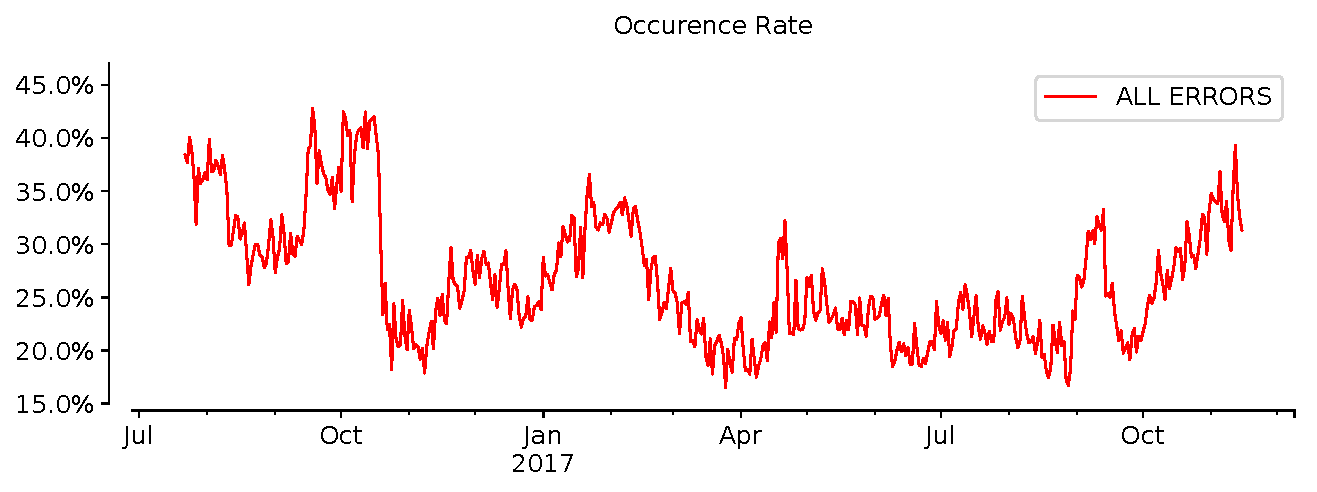
\includegraphics[keepaspectratio, height=5cm, width=15cm]{figures/errors/netflix-occurence-rate-timeseries-all-errors.pdf}
	\caption[Error Occurrence Rate for All Errors]{Error occurrence rate for all errors during the whole timeline. The occurrence rate mostly lies between 15\%-45\% for a single day.}
	\label{fig:Occurrence Rate All Errors}
\end{figure}
\begin{figure}[!ht]
	\centering
	\begin{minipage}{0.45\textwidth}
		\centering
		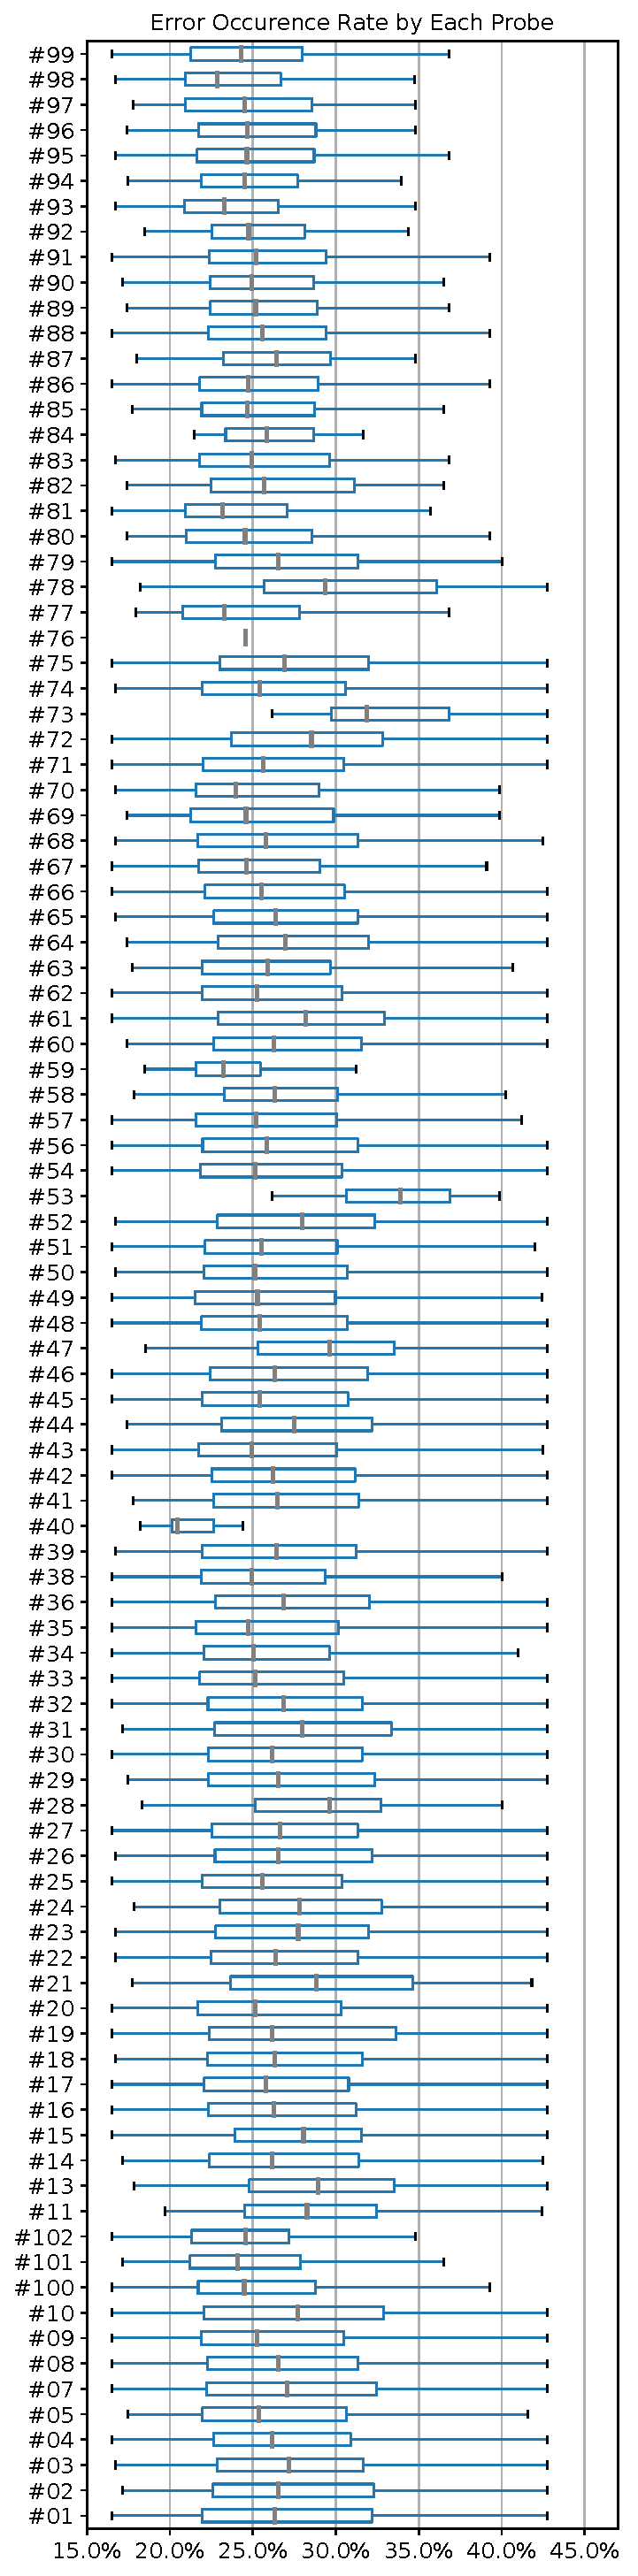
\includegraphics[keepaspectratio, height=18cm, width=15cm]{figures/errors/netflix-occurence-rate-all-errors-boxplots-vert.pdf}
		\caption[Error Occurrence Rate by Each Probe]{(a)}
	\end{minipage}
	\begin{minipage}{0.45\textwidth}
		\centering
		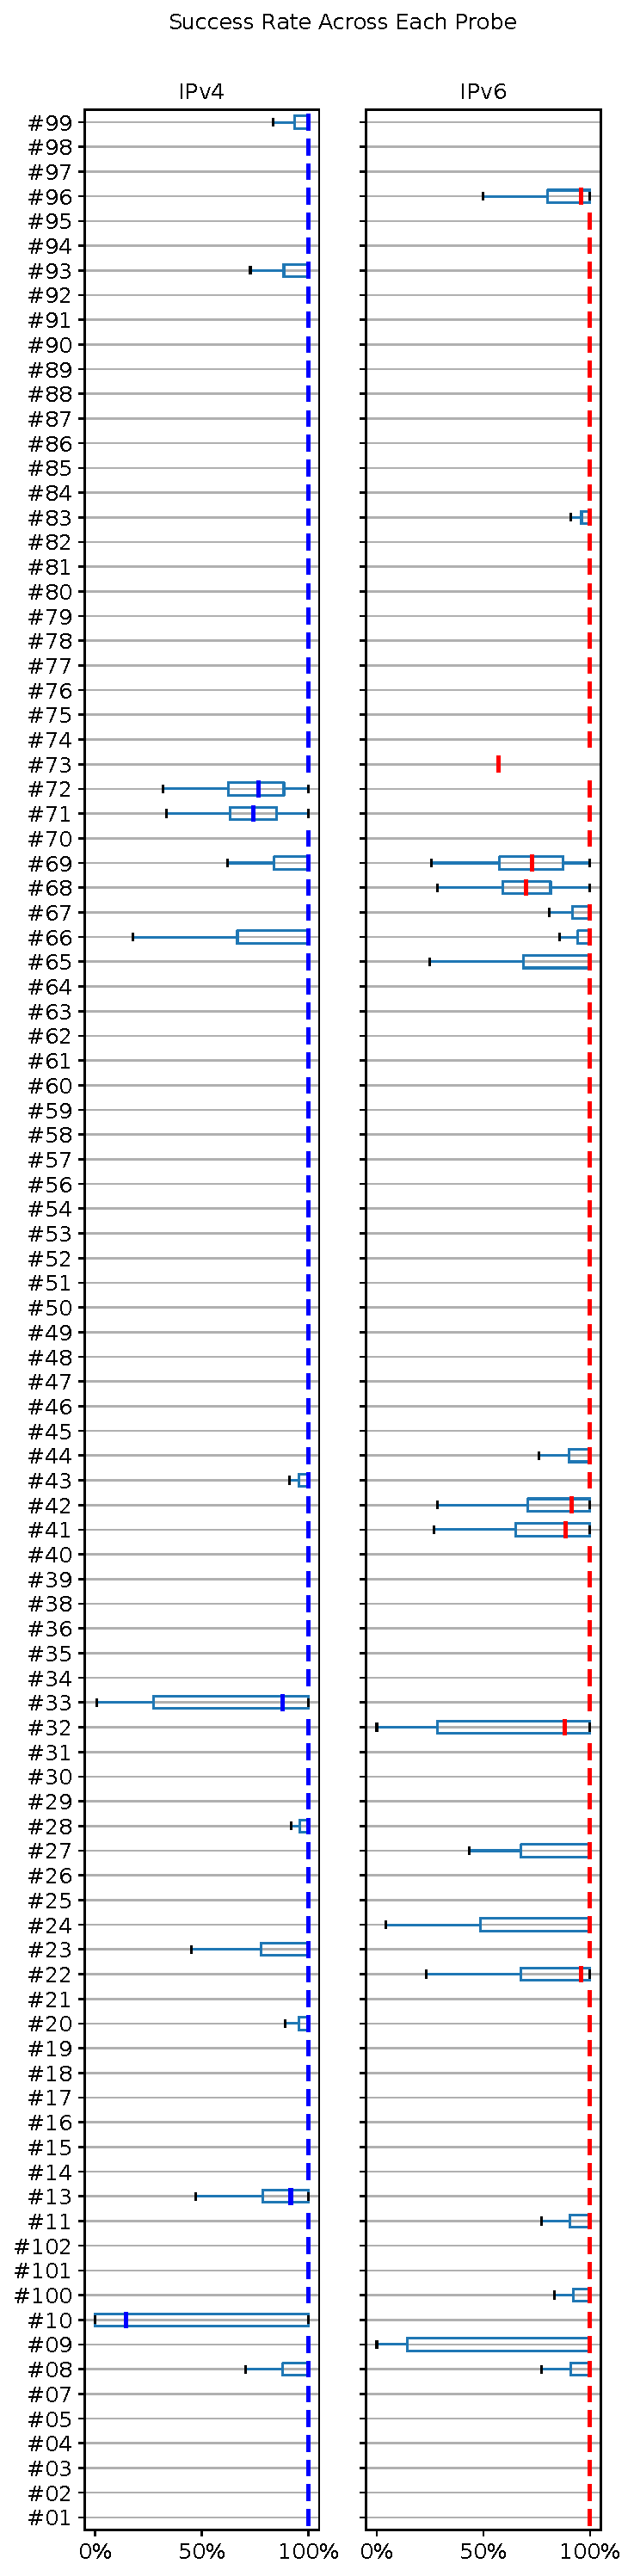
\includegraphics[keepaspectratio, height=18cm, width=15cm]{figures/success/netflix-success-rate-boxplot-each-probe-vert.pdf}
		\caption[Success Rate by Each Probe]{(b)}
	\end{minipage}
	\caption[Error Occurrence and Success Rate by Each Probe]{(a) Boxplot of error occurrence rate for each probe. It signifies that the error occurrence rate is evenly distributed across each probe. (b) Boxplots of success rate across each probe over IPv4 and IPv6. Around 30 probes have varying success rate.}
	\label{fig:Error Occurrence and Success Rate by Each Probe}
\end{figure}

\FloatBarrier

\subsection*{\textit{Success Rate}}
\begin{figure}[!ht]
	\centering
	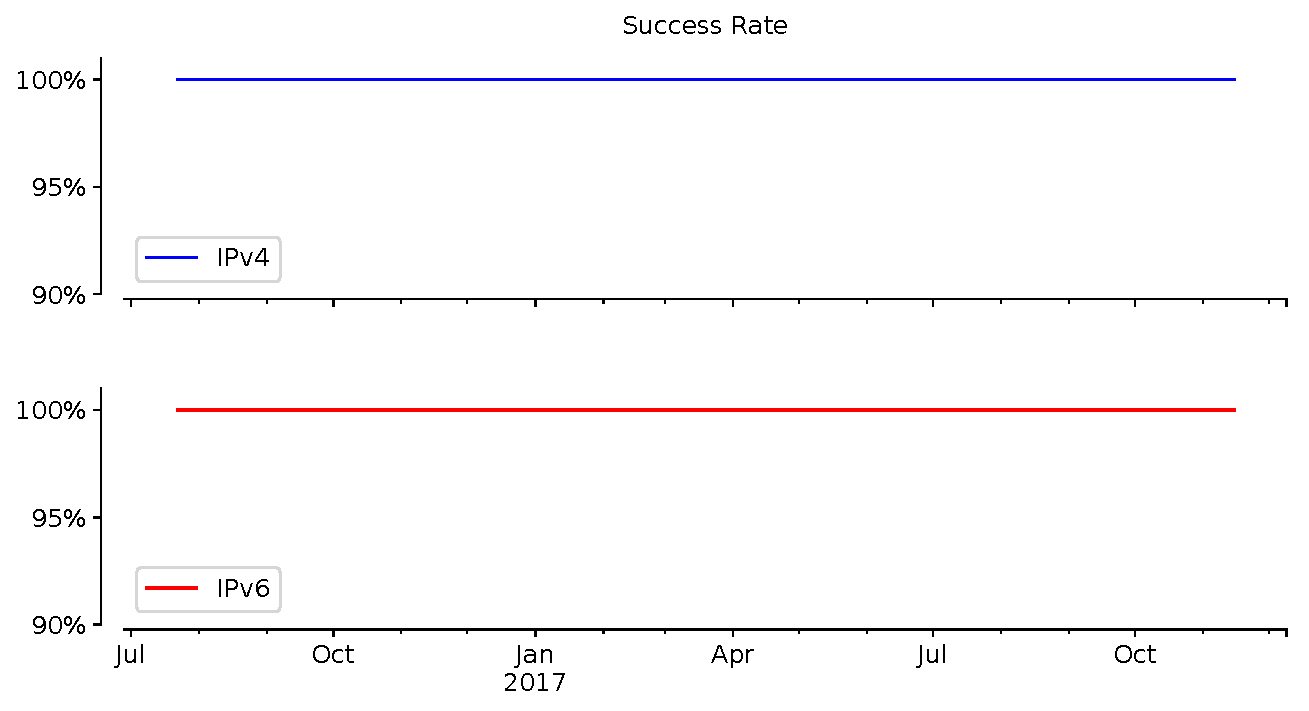
\includegraphics[keepaspectratio, height=5cm, width=15cm]{figures/success/netflix-success-rate-timeseries.pdf}
	\caption[Success Rate Timeseries]{Time series of success rate over IPv4 and IPv6. We are taking the median aggregate of success rate across all the probes on each day since July, 2016. Median Success rate for both the address families remains constant around 100\% over the entire time duration.}
	\label{fig:Success Rate Timeseries}
\end{figure}
\begin{figure}[!ht]
	\centering
	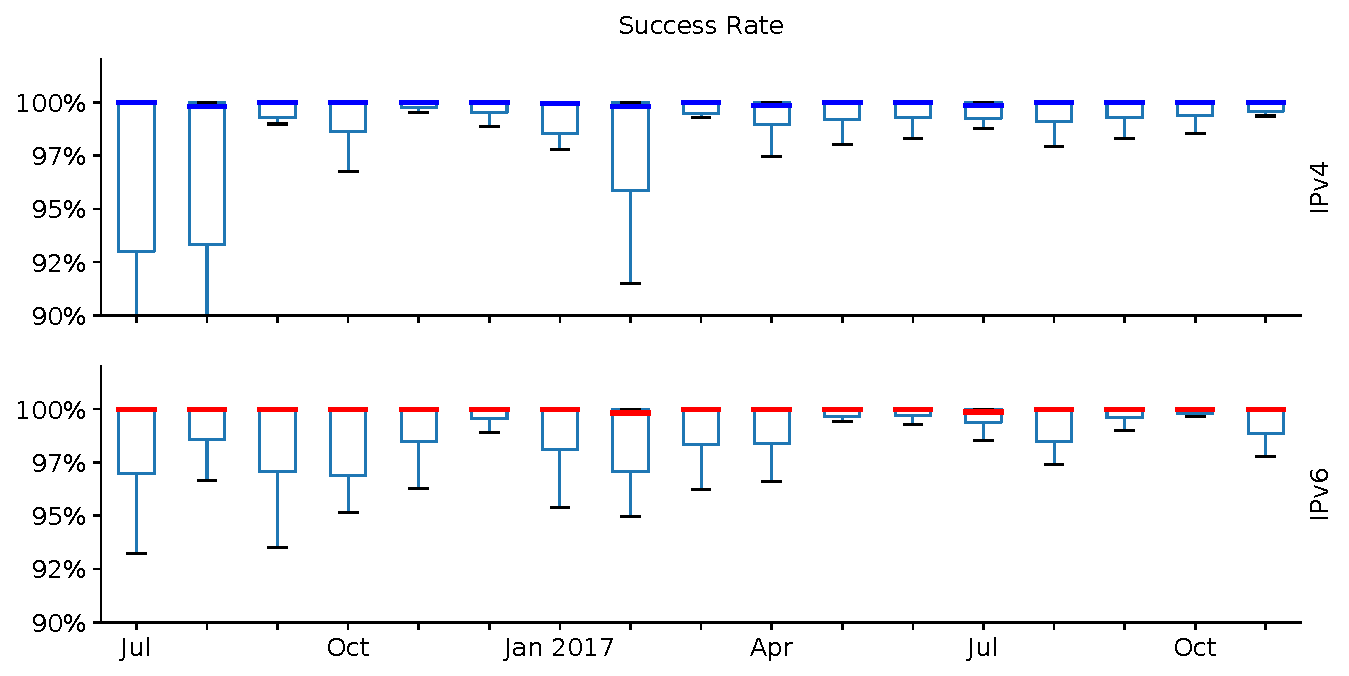
\includegraphics[keepaspectratio, height=5cm, width=15cm]{figures/success/netflix-success-rate-boxplot.pdf}
	\caption[Success Rate Boxplot per Month]{Boxplot of success rate over IPv4 and IPv6. The median line is close to 100\% for both the address families and resembles the \cref{fig:Success Rate Timeseries}. Variation among different months can be seen here.}
	\label{fig:Success Rate Boxplot}
\end{figure}
After considering the error rate, it would be goood to look at the success of the test. We will now consider the success rate over both the address families i.e. IPv4 and IPv6.
For success rate we will be considering the \textit{successes} field, described in the \cref{table:netflix} in \cref{chapter:Datasets}. We will start with the similar analysis Vaibhav Bajpai et al. did in \cite{bajpaimeasuring}.
They define success rate as the successful cases upon the total number of cases in the dataset. Downloading a stall free version of the video indicates a successful test, and if a stall occurs
the test restarts by stepping down to a lower bitrate and reports an error. Thus, we are not considering the cases where this is a stall i.e. we are excluding cases when the \textit{error} is "STALLED\_WILL\_STEP\_DOWN" and "STALLED\_ON\_FINAL". 
\cref{fig:Success Rate Timeseries} shows us the time series of median success rates across all the probes on each day since July, 2016, when there isn't a stall. As we can see from the plot, 
median success rate remain constant around 100\% for both the address families.

\begin{figure}[!ht]
	\centering
	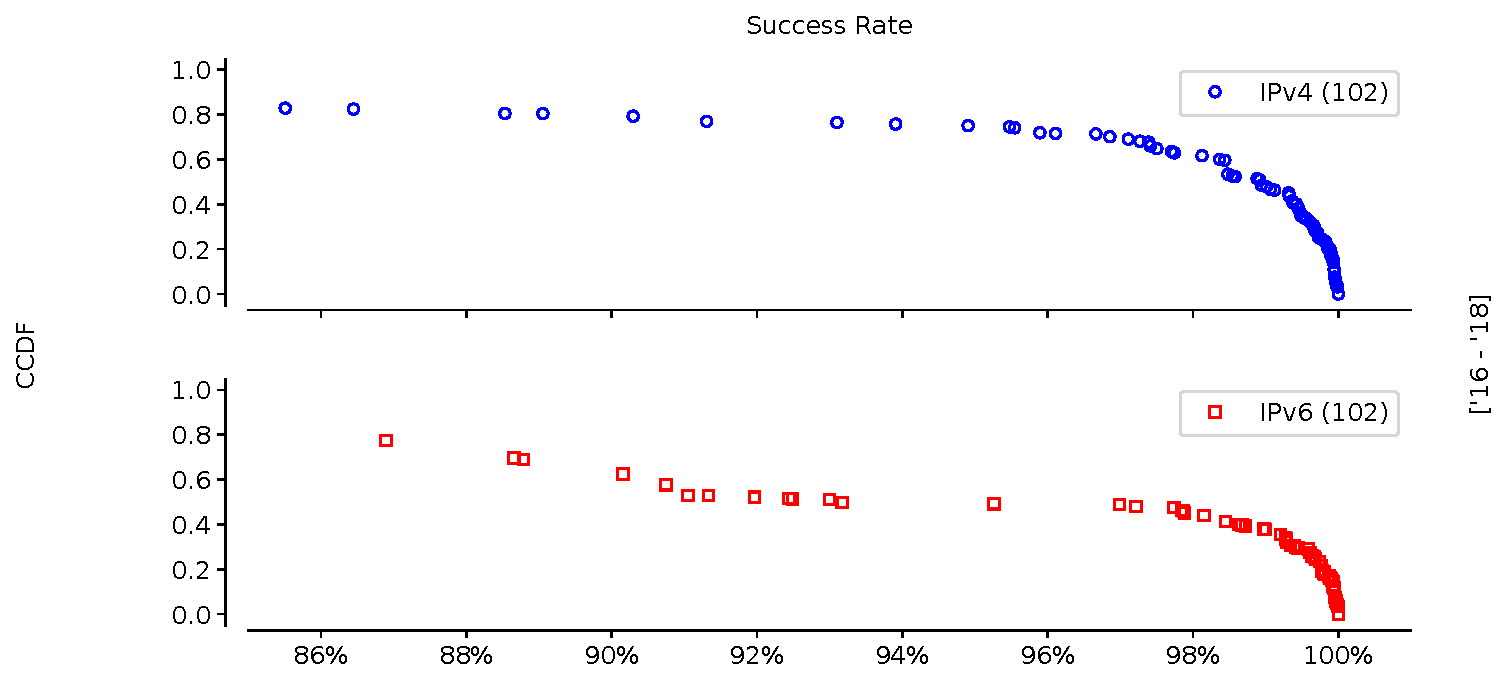
\includegraphics[keepaspectratio, height=5cm, width=15cm]{figures/success/netflix-success-rate-ccdf.pdf}
	\caption[Success Rate CCDF]{CCDF of success rate over IPv4 and IPv6, when there isn't a stall. Around 79\% of the probes achieve success rate of more than 90\% for IPv4, while for IPv6, only around 63\% of the probes were able to achieve this success rate.}
	\label{fig:Success Rate CCDF}
\end{figure}

Median aggregate ensures that the results doesn't get biased due to a specific probe or specific vantage point. We also plotted all the datapoints and not just the medians, and the results can be seen in \hyperref[chapter:appdataset]{Appendices}.
To further investigate the success rate we plotted the boxplots to see the variation among different months.
We have rounded the time to the nearest month, and we can see in \cref{fig:Success Rate Boxplot} that the median success rate is close to 100\% for both the address families but the individual distribution varies across time.
We further investigate the distribution of success rate over IPv4 and IPv6, when there isn't a stall. We calculated the success rate and then took the CCDF of it. 
\cref{fig:Success Rate CCDF} shows the CCDF of success rate over IPv4 and IPv6. Around 79\% of the probes achieve success rate of more than 90\% for IPv4, while for IPv6, only around 63\% of the probes were able to achieve this success rate. It can be seen that probes
achieve a lower success rate over IPv6. On careful investigation, we found out that the reason for lower success rates over IPv6 is due to DNS Resolution Error and Network Errors. Moving forward we will work on cases where both the address
families reports success. \hyperref[chapter:appdataset]{Appendices} also discusses the CDF for two individual months i.e. August 2016 and October 2017. 
We also calcualted the success rate across each probe. \cref{fig:Error Occurrence and Success Rate by Each Probe}(b) gives us the bocplot of success rate over IPv4 and IPv6 across each probe. 
We can see from the median values that there are around 30 probes which have varying success rate over the time line. We did time series analysis of success rate across IPv4 and IPv6 removing these outliers and the results
can be seen in the \hyperref[chapter:appdataset]{Appendices}.

\FloatBarrier
\subsection*{\textit{Success Rate by Region}}
\begin{table}[!h]
	\centering
	\caption{Regions with Number of Probes}
	\label{table:regions}
	\begin{tabular}{lp{2cm}}
  		\toprule
  		\textbf{Regions} & \textbf{\#Probes} \\ 
  		\midrule
  		European Region & 60 \\ 
  		Region of the Americas & 32 \\
  		Western Pacific Region & 9 \\
  		African Region & 1 \\
  		\bottomrule
\end{tabular}
\end{table}
\begin{figure}[!ht]
	\begin{minipage}{0.5\textwidth}
		\centering
		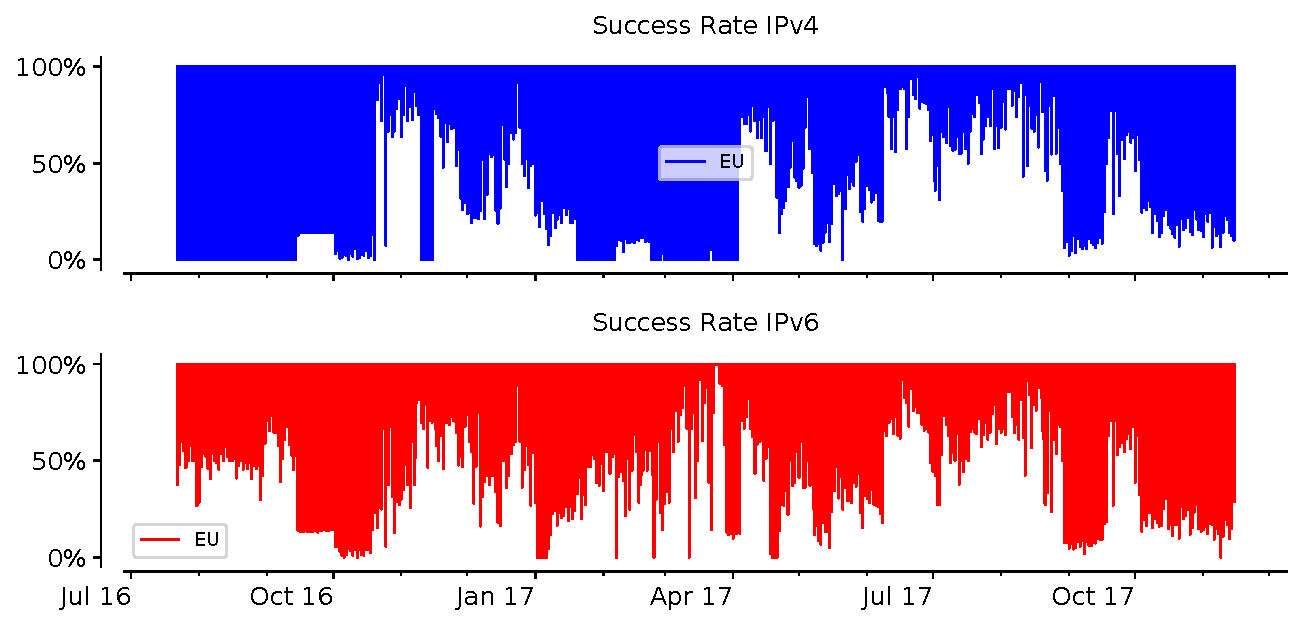
\includegraphics[keepaspectratio, height=4cm, width=15cm]{figures/success/netflix-success-rate-timeseries-region-eu.pdf}
		\caption[Time series of success rate over IPv4 and IPv6 for European Region]{(a)}
	\end{minipage}
	\begin{minipage}{0.5\textwidth}
		\centering
		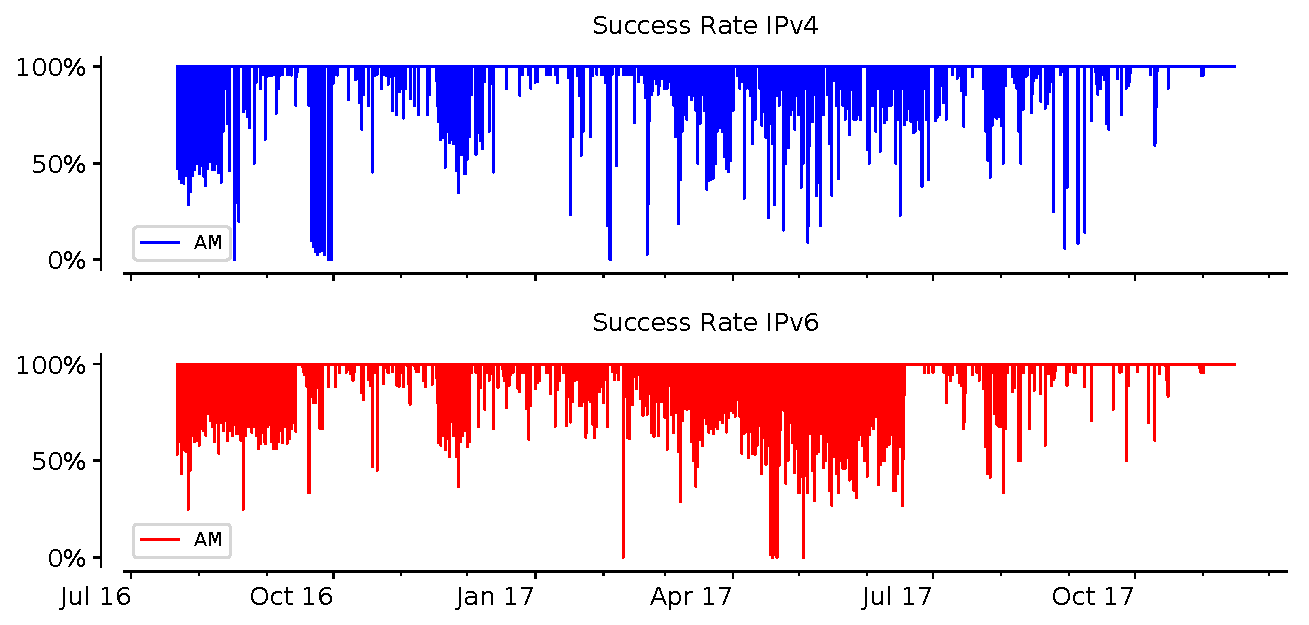
\includegraphics[keepaspectratio, height=4cm, width=15cm]{figures/success/netflix-success-rate-timeseries-region-am.pdf}
		\caption[Time series of success rate over IPv4 and IPv6 for Region of Americas]{(b)}
	\end{minipage}
	\begin{minipage}{0.5\textwidth}
		\centering
		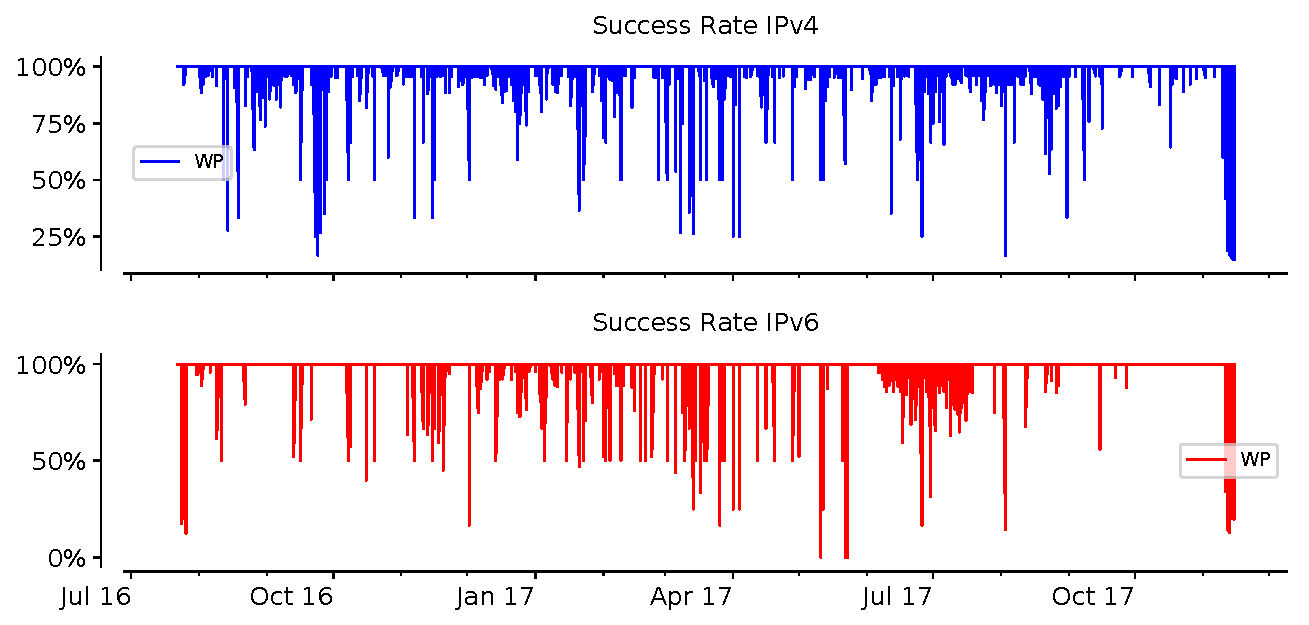
\includegraphics[keepaspectratio, height=4cm, width=15cm]{figures/success/netflix-success-rate-timeseries-region-wp.pdf}
		\caption[Time series of success rate over IPv4 and IPv6 for Western Pacific Region]{(c)}
	\end{minipage}
	\begin{minipage}{0.5\textwidth}
		\centering
		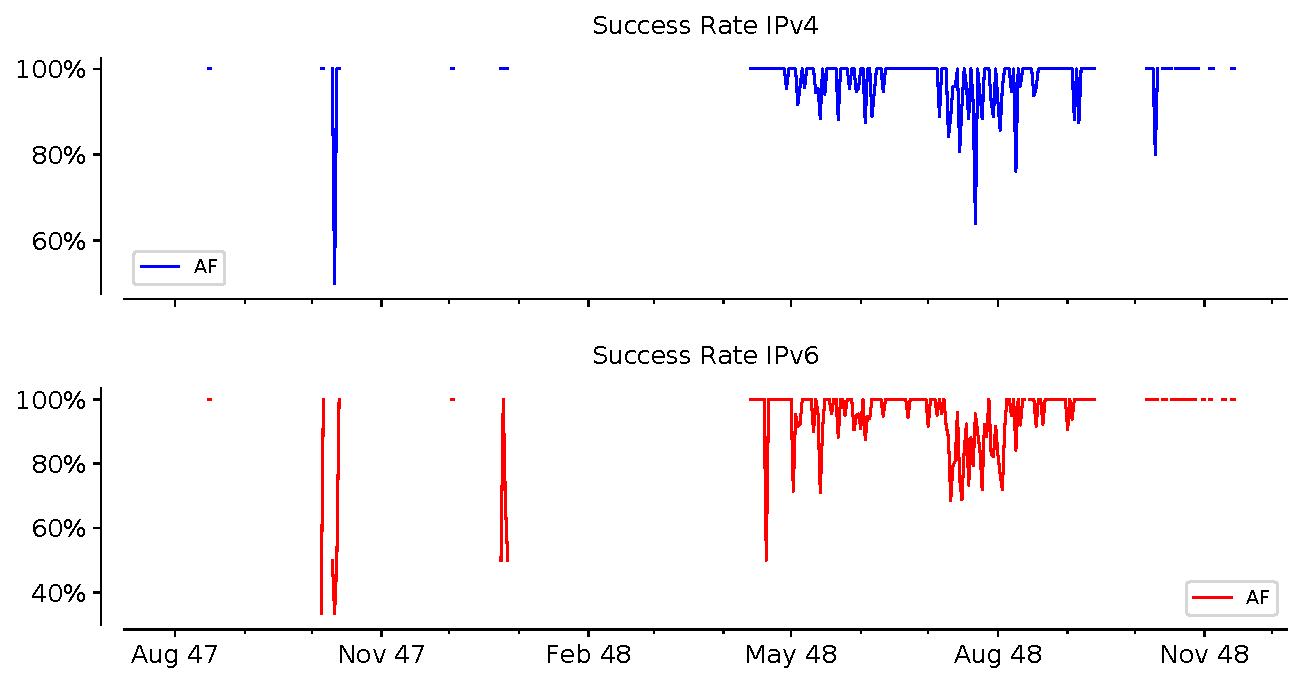
\includegraphics[keepaspectratio, height=4cm, width=15cm]{figures/success/netflix-success-rate-timeseries-region-af.pdf}
		\caption[Time series of success rate over IPv4 and IPv6 for African Region]{(d)}
	\end{minipage}
	\caption[Timeseries of Success rate over IPv4 and IPv6 for different regions]{(a) Time series of success rate over IPv4 and IPv6 for European Region, (b) Time series of success rate over IPv4 and IPv6 for Region of Americas,
(c) Time series of success rate over IPv4 and IPv6 for Western Pacific Region, (d) Time series of success rate over IPv4 and IPv6 for African Region. We can see the variation of success rate among different regions. Success rate in Region of Americas seems to quite better compared to European Region.}
	\label{fig:Timeseries of Success rate over IPv4 and IPv6 for different regions}
\end{figure}
We wanted to see how success rate over IPv4 and IPv6 performs by different geographical regions of the world. The metadata of the probes is listed at \cite{metadata}, 
provides us the geographical information of the probes as well.
There is a \textit{location} field in the metadata which tells us the city or organisation where the probe is located. We did some manual analysis and collected the 
different regions based on this \textit{location} field.
We then created a new field named \textit{region} containing the geographical region where the probe is located, based on the World Health Organization defination of 
different geographical regions of the world \cite{whoregions}.
\cref{table:regions} gives the number of SaKnows probes in different regions of the world. The probes are situated in four different regions. 
\begin{figure}[!ht]
	\centering
	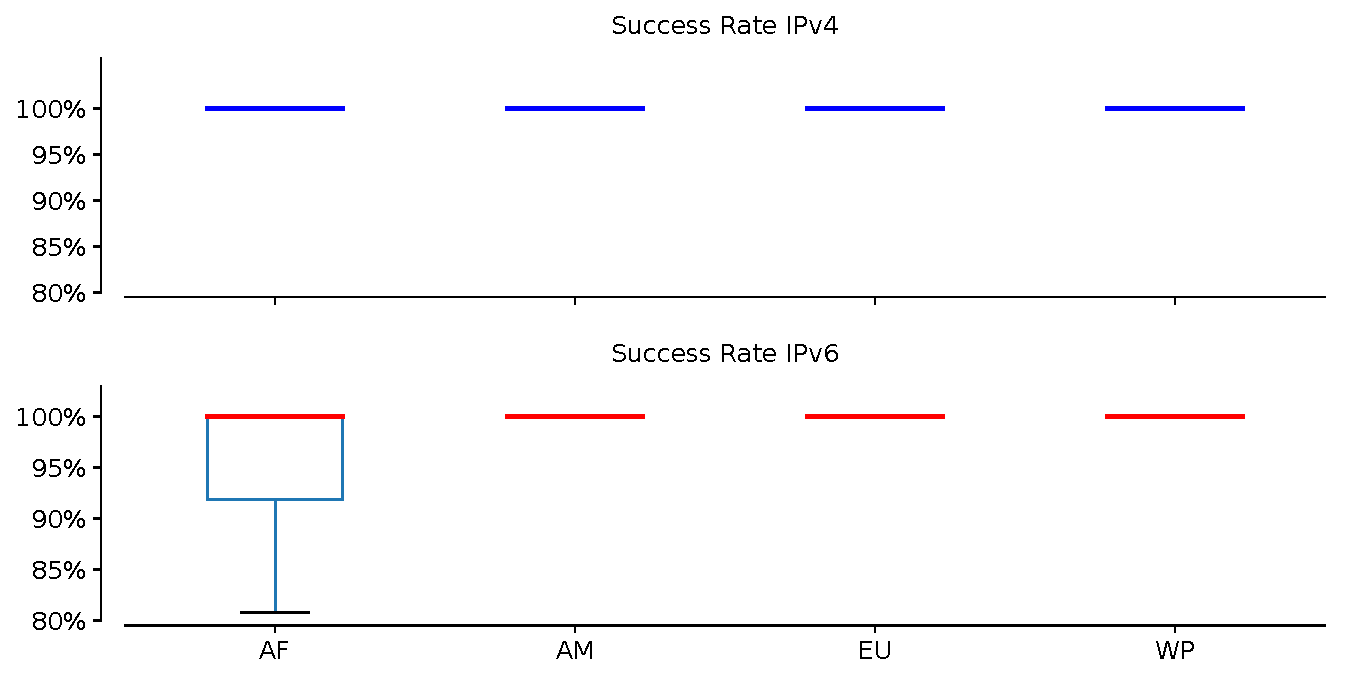
\includegraphics[keepaspectratio, height=4cm, width=15cm]{figures/success/netflix-success-rate-boxplot-region.pdf}
	\caption[Success Rate Boxplot for different Regions]{Boxplot of success rate over IPv4 and IPv6 for different regions. The performance over IPv4 and IPv6 seems equivalent for different regions, except for African region where first quartile of success rate is around 80\%. }
	\label{fig:Success Rate Boxplot for Different Regions}
\end{figure}
\begin{figure}[!ht]
	\centering
	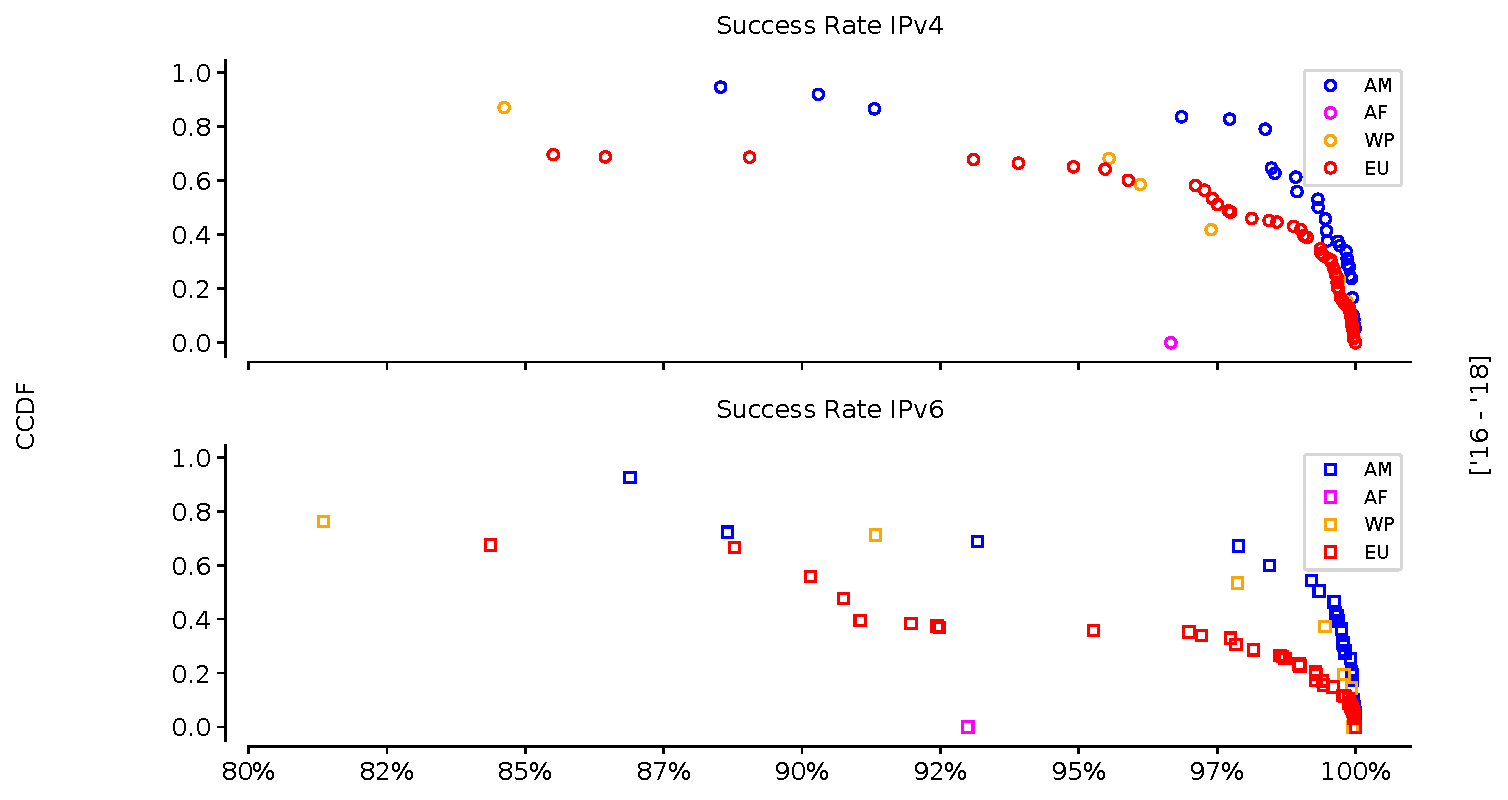
\includegraphics[keepaspectratio, height=4cm, width=15cm]{figures/success/netflix-success-rate-ccdf-region.pdf}
	\caption[Success Rate CCDF for Different Regions]{CCDF of success rate over IPv4 and IPv6 for different regions. The success rate for Region of the Americas is better than European Region over both the address families.}
	\label{fig:Success Rate CCDF for Different Regions}
\end{figure}
We followed the same steps as what we did in the previous section. Here, we merged the \textit{region} field based on the name of the probe. After merging we grouped the data based on \textit{dtime},
\textit{address family (af)}, \textit{probe name} and \textit{region}, aggregating the \textit{success} field based on this grouping. We then simply calcualted the success rate for all these regions
and then plotted them as a time series. \cref{fig:Timeseries of Success rate over IPv4 and IPv6 for different regions} gives the time series of success rate over IPv4 and IPv6 for different regions, and as can be seen Success rate in Region of Americas seems to quite better compared to European Region.
To further investigate we plotted the boxplot of success rate over IPv4 and IPv6 for different regions in \cref{fig:Success Rate Boxplot for Different Regions}.The performance over IPv4 and IPv6 seems equivalent for different regions, except for African region where first quartile of success rate is around 80\%.
We wanted to see the distribution of success rate over IPv4 and IPv6 for these regions. \cref{fig:Success Rate CCDF for Different Regions} gives the CCDF of success rate over IPv4 and IPv6 for different regions. We can see that the success rate for Region of the Americas is better than European Region over both the address families.
\FloatBarrier

\subsection*{\textit{Success Rate by Network Type}}
\begin{table}[!h]
	\centering
	\caption{Network Types with Number of Probes}
	\label{table:regions}
	\begin{tabular}{lp{2cm}}
  		\toprule
  		\textbf{Network Type} & \textbf{\#Probes} \\ 
  		\midrule
  		RESIDENTIAL & 79 \\ 
  		NREN & 8 \\
  		RESEARCH & 2 \\
  		BUSINESS & 5 \\
		DATACENTER & 3 \\
  		OPERATOR LAB & 4 \\
		IXP & 1 \\
  		\bottomrule
\end{tabular}
\end{table}

After going through the success rate for different geographical regions, we also wanted to see the success rate over IPv4 and IPv6 for different network types. 
There is a \textit{Type} field in the metadata of the probes \cite{metadata}, which
gives us the network type of the probe. There are seven different types listed in the metadata and \cref{table:types} shows us these seven network types and the 
number of probes in each type. As can be seen most of the probes are "RESIDENTIAL" probes.
Also, we grouped the "NREN" and "RESEARCH" together into "RESEARCH", and "BUSINESS" and "DATACENTER" into "BUSINESS" as per \cite{bajpaimeasuring}. We created a 
new field named \textit{type} and merged this field based on the \textit{name} of the probe.
Here, we are grouping on \textit{dtime}, \textit{address family (af)}, \textit{probe} and \textit{type} field. We then simply calculated the \textit{success rate} 
over IPv4 and IPv6 for different network types and plotted them as a time series. \cref{fig:Timeseries of Success rate over IPv4 and IPv6 for different Network Type} shows
the timeseries of success rate over IPv4 and IPv6 for different network types, and we can see that the "RESIDENTIAL" probes are influencing the success rate over 
IPv4 and IPv6 across all probes \cref{fig:Success Rate Timeseries}.

\begin{figure}[!ht]
	\begin{minipage}{0.5\textwidth}
		\centering
		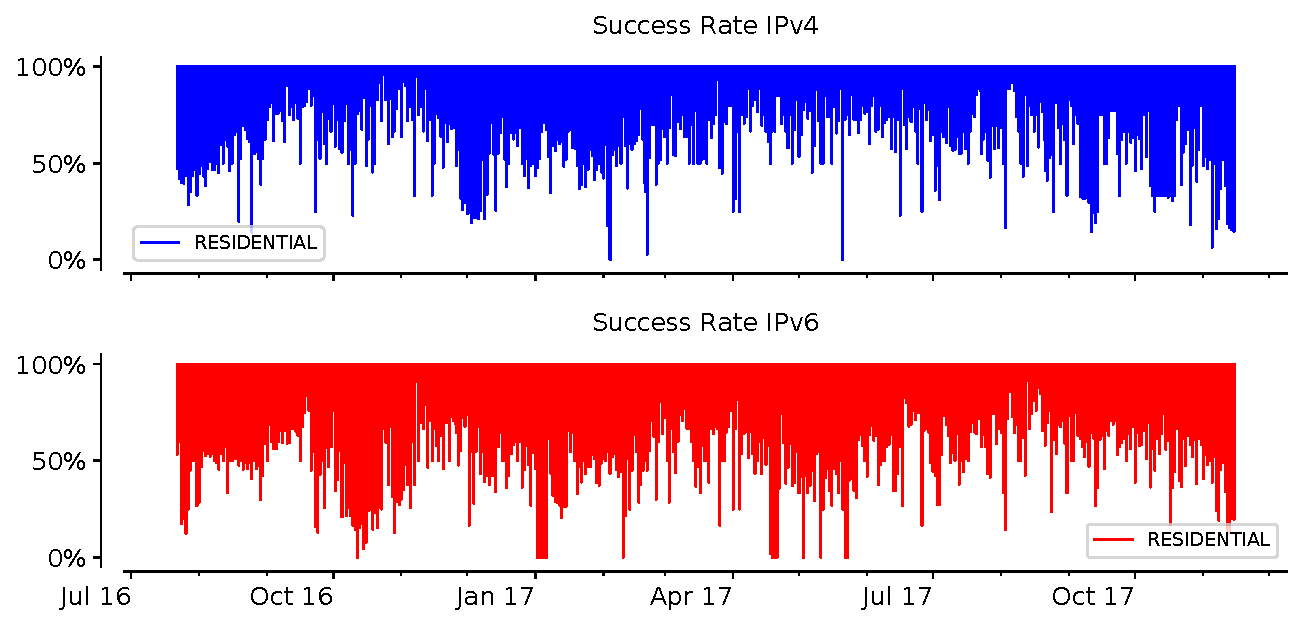
\includegraphics[keepaspectratio, height=4cm, width=10cm]{figures/success/netflix-success-rate-timeseries-network-type-resd.pdf}
		\caption[Timeseries of Success rate over IPv4 and IPv6 as per Residential Probes]{(a)}
	\end{minipage}
	\begin{minipage}{0.5\textwidth}
		\centering
		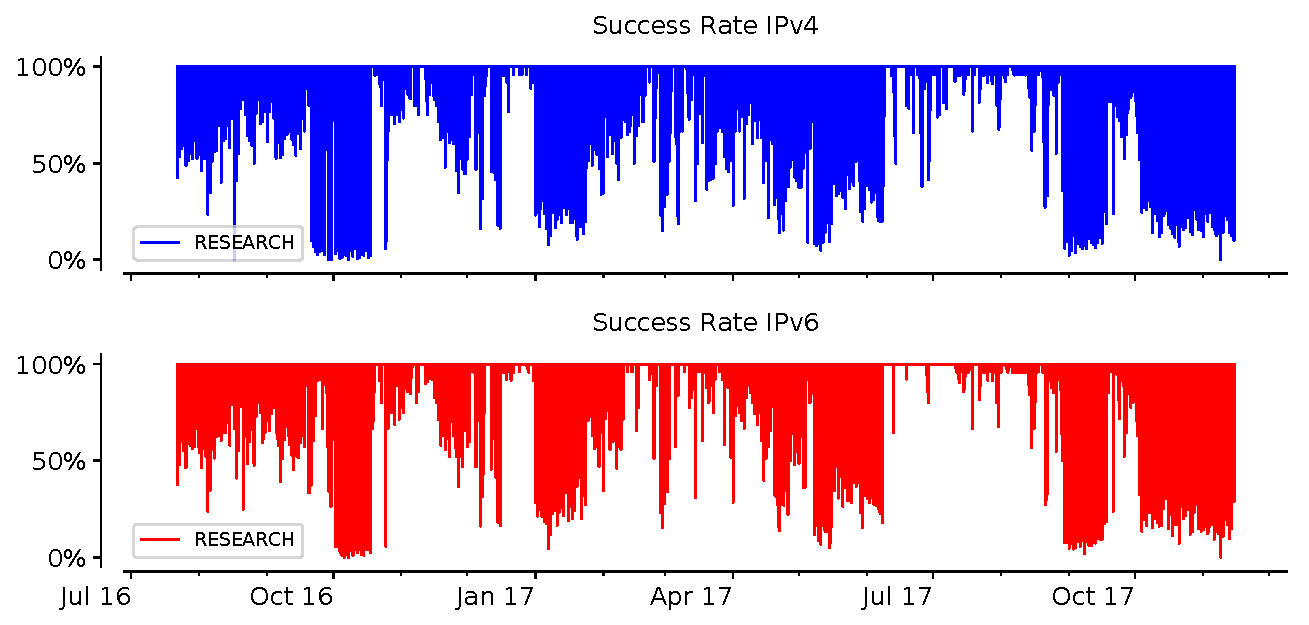
\includegraphics[keepaspectratio, height=4cm, width=10cm]{figures/success/netflix-success-rate-timeseries-network-type-nren.pdf}
		\caption[Timeseries of Success rate over IPv4 and IPv6 as per Research Probes]{(b)}
	\end{minipage}
	\begin{minipage}{0.5\textwidth}
		\centering
		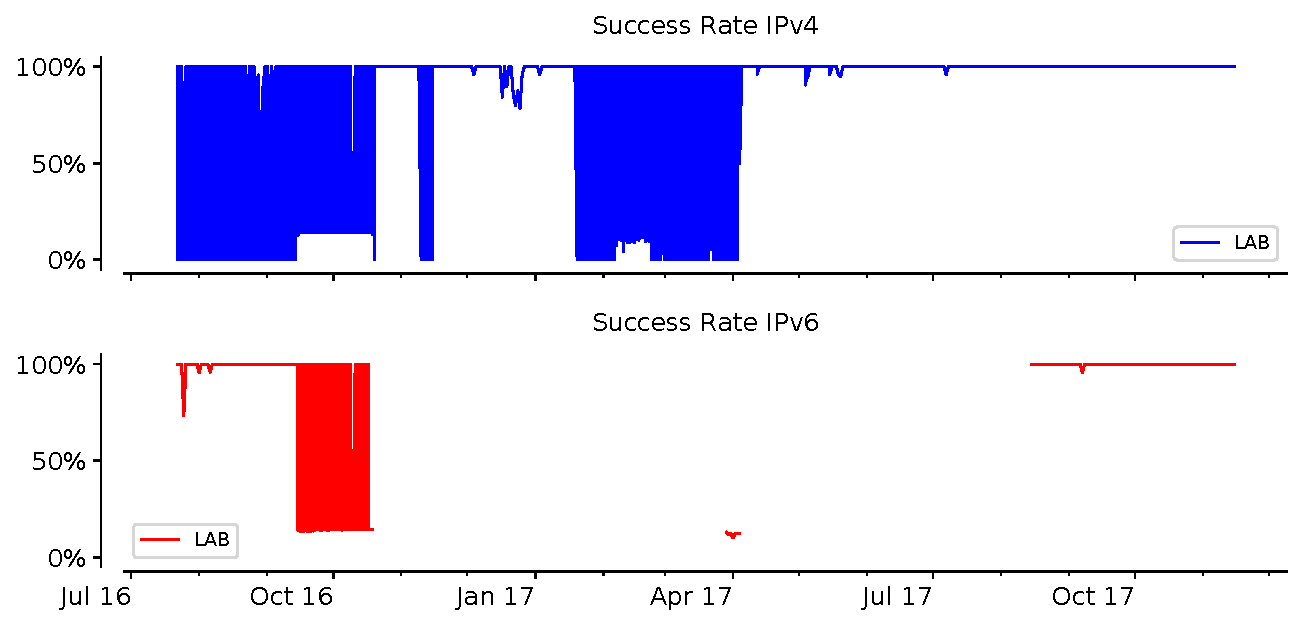
\includegraphics[keepaspectratio, height=4cm, width=10cm]{figures/success/netflix-success-rate-timeseries-network-type-lab.pdf}
		\caption[Timeseries of Success rate over IPv4 and IPv6 as per Lab Probes]{(c)}
	\end{minipage}
	\begin{minipage}{0.5\textwidth}
		\centering
		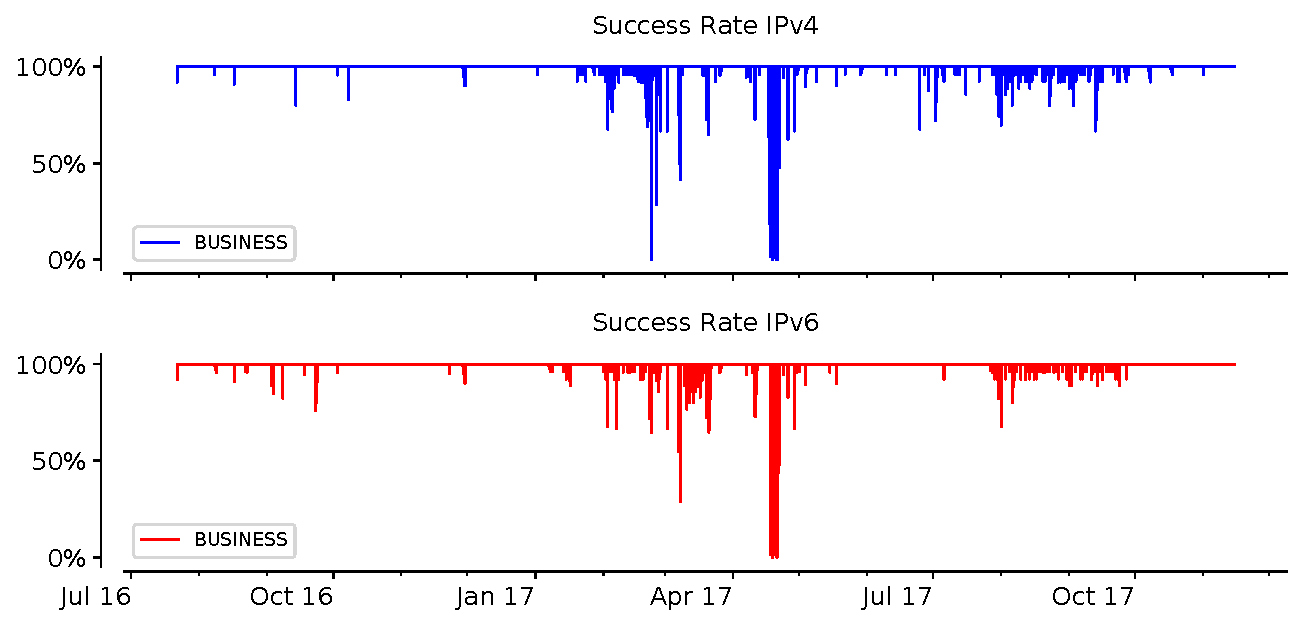
\includegraphics[keepaspectratio, height=4cm, width=10cm]{figures/success/netflix-success-rate-timeseries-network-type-bus.pdf}
		\caption[Timeseries of Success rate over IPv4 and IPv6 as per Business Probes]{(d)}
	\end{minipage}
	\begin{minipage}{0.5\textwidth}
		\centering
		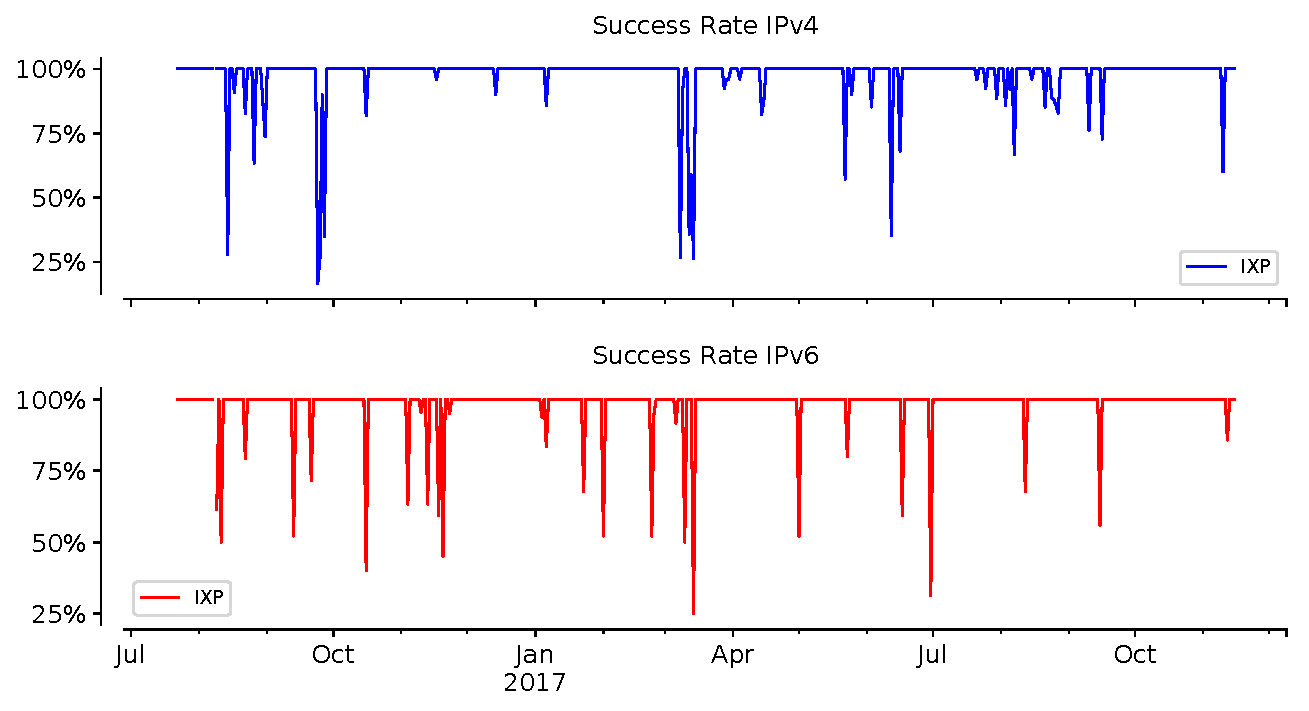
\includegraphics[keepaspectratio, height=4cm, width=10cm]{figures/success/netflix-success-rate-timeseries-network-type-ixp.pdf}
		\caption[Timeseries of Success rate over IPv4 and IPv6 as per IXP Probe]{(e)}
	\end{minipage}
	\caption[Timeseries of Success rate over IPv4 and IPv6 as per different network types]{(a) Time series of success rate over IPv4 and IPv6 for RESIDENTIAL Probes, (b) Time series of success rate over IPv4 and IPv6 for RESEARCH Probes,
(c) Time series of success rate over IPv4 and IPv6 for LAB Probes, (d) Time series of success rate over IPv4 and IPv6 for BUSINESS Probes. (e) Time series of success rate over IPv4 and IPv6 for IXP Probes. We can see the variation of success rate among different regions. Success rate in Region of Americas seems to quite better compared to European Region.}
	\label{fig:Timeseries of Success rate over IPv4 and IPv6 for different Network Type}
\end{figure}
\begin{figure}[!ht]
	\centering
	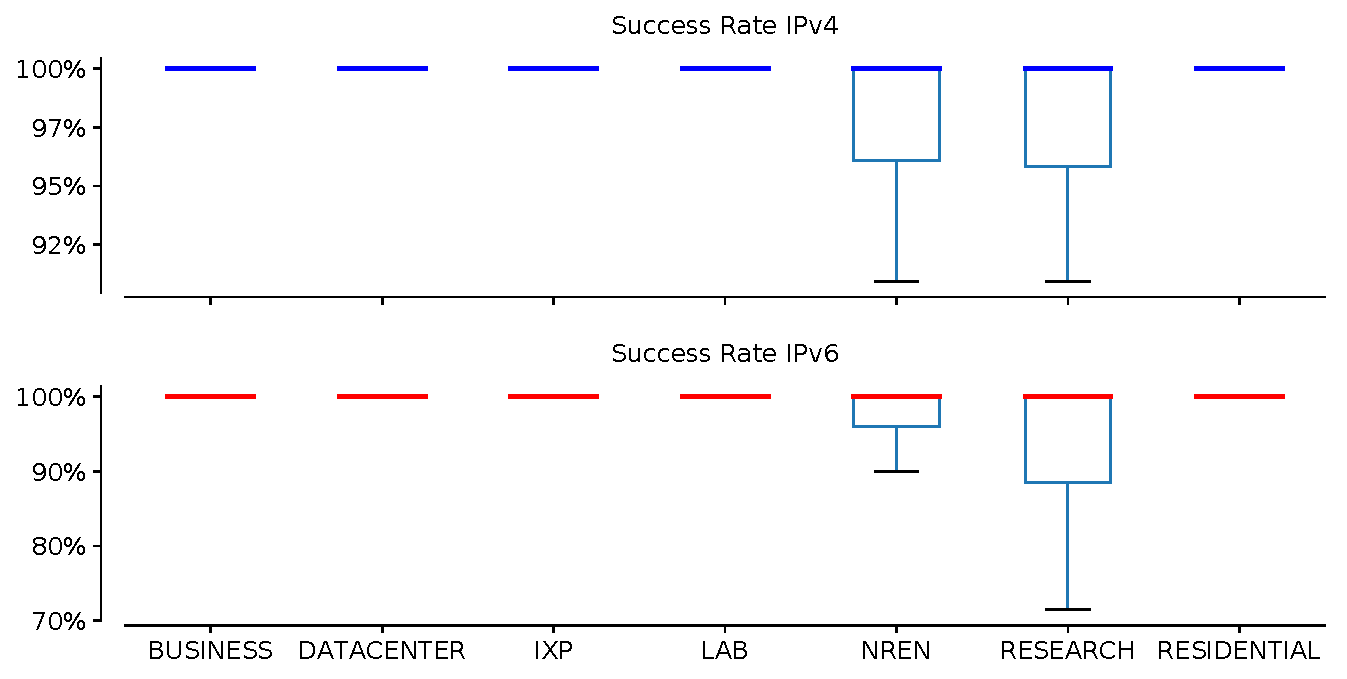
\includegraphics[keepaspectratio, height=4cm, width=15cm]{figures/success/netflix-success-rate-boxplot-type.pdf}
	\caption{Success Rate Boxplot per each Network Types of Probes}
	\label{fig:Success Rate Boxplot per each Network Types of Probes}
\end{figure}
To further investigate, we plotted the boxplot of success rate over IPv4 and IPv6 for different network types in \cref{fig:Success Rate Boxplot per each Network 
Types of Probes}. It can be seen that boxplot of usccess rate is around 100\% over IPv4 and IPv6, except "NREN" and "RESEARCH" probes 
where the success rate is distributed. We also wanted to see the distribution of success rate over both the address families for different network types. 
\cref{fig:Success Rate CCDF for probes over different Network Types} gives us the CCDF of success rate over both families for the probes in different
network types. CCDF of success rate for "RESIDENTIAL" probes resembles the CCDF of success rate across all probes as in \cref{fig:Success Rate CCDF}.
\begin{figure}[!ht]
	\centering
	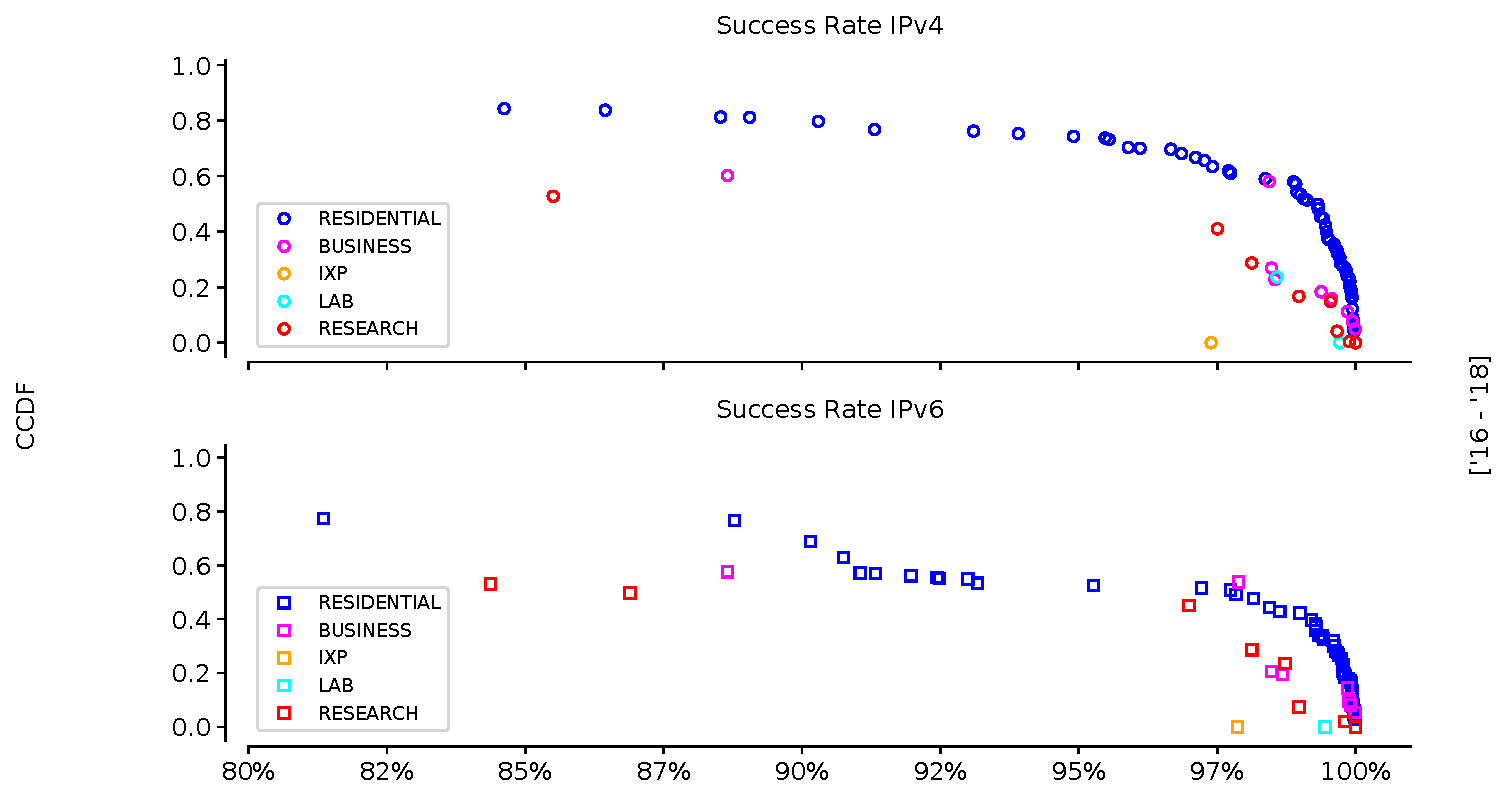
\includegraphics[keepaspectratio, height=4cm, width=15cm]{figures/success/netflix-success-rate-ccdf-type.pdf}
	\caption{Success Rate CCDF for probes over different Network Types}
	\label{fig:Success Rate CCDF for probes over different Network Types}
\end{figure}
\vfill
\FloatBarrier

\section{IPv6 Preference}\label{chapter:ipv6preference}
\begin{figure}[!ht]
	\centering
	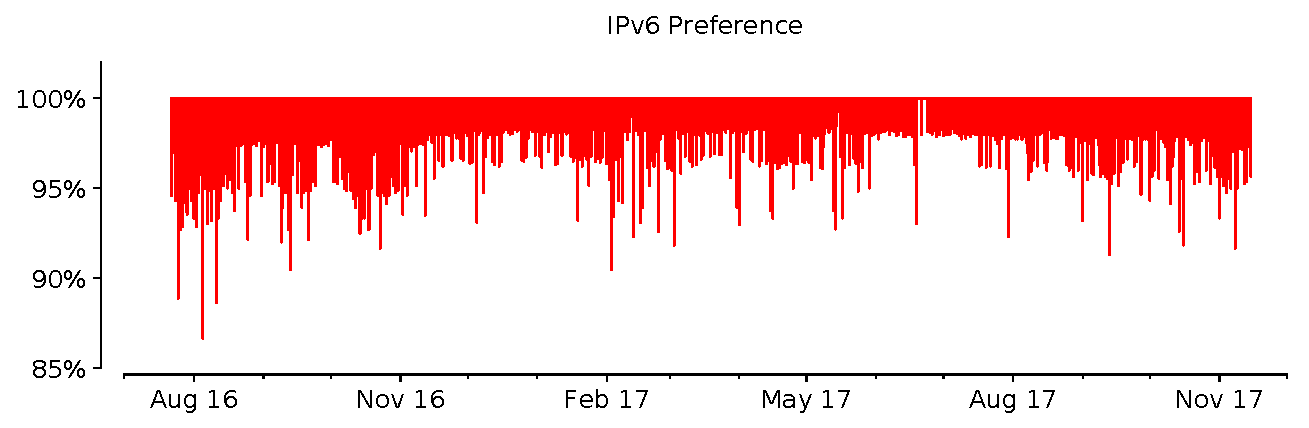
\includegraphics[keepaspectratio, height=4cm, width=15cm]{figures/preference/he-preference-timeseries.pdf}
	\caption[IPv6 Preference Timeseries]{The timeseries shows the effects of HE algorithm and as per this the TCP connections were preferred for more than 90\% of the time during the whole time period of the dataset.}
	\label{fig:IPv6 Preference Timeseries}
\end{figure}
\begin{figure}[!ht]
	\centering
	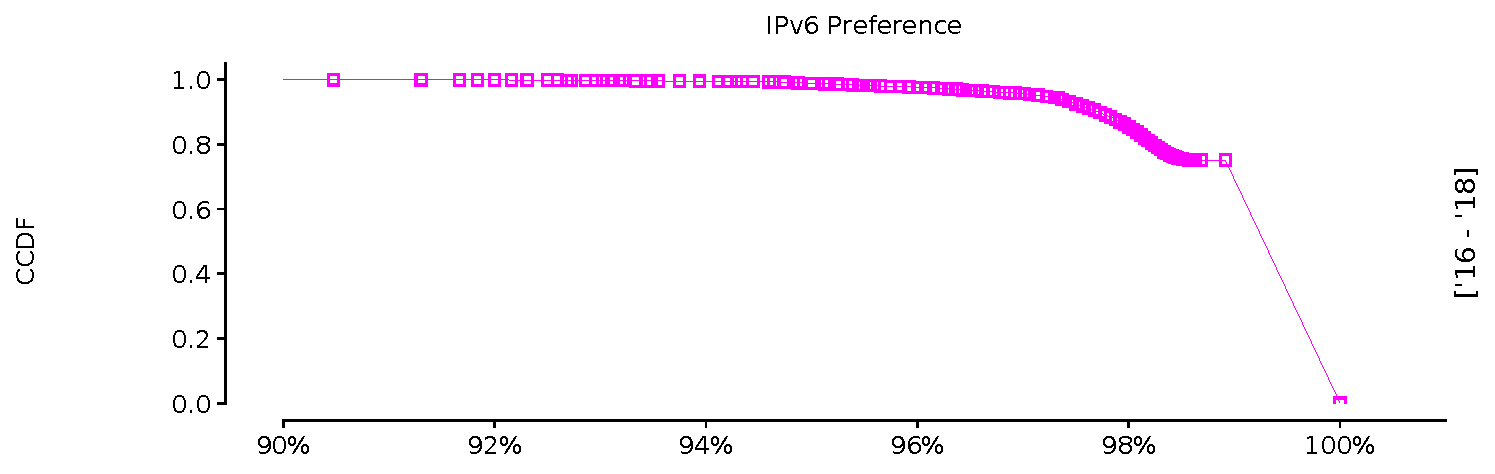
\includegraphics[keepaspectratio, height=4cm, width=15cm]{figures/preference/he-preference-ccdf.pdf}
	\caption[IPv6 Perference CCDF]{CCDF of TCP connection establishment preference over IPv6. The TCP connections over IPv6 to the OCA server are preferred around 93\% of the time.}
	\label{fig:IPv6 Preference CCDF}
\end{figure}

We are measuring TCP connect times (\textit{connect\_time} field in the table \ref{table: netflix}) to the Netflix Open Connect Appliance (OCA) server in (refer Sequence diagram here). Vaibhav Bajpai et al. in \cite{bajpaimeasuring} measured the TCP connect times for Youtube, and we followed their analysis approach here. TCP connect times doesn't consider the DNS name resolution time, and is based on the connect() system call completion time. 
We are doing this as applications running on dual-stacked hosts should prefer connections over IPv6, as per the default address selection policy for IPv6 \cite{rfc6724}. 
RFC 6724 makes getaddrinfo() resolve DNS names in an order that mandates an IPv6 upgrade path for the applications, whereas, Happy Eyeballs (HE) algorithm \cite{rfc6555} allows these applications to resolve to IPv4 if the connectivity over IPv6 is not good. As per HE algorithm the connectivity is not considered good when the connection does not complete within 300 ms. We first filtered the data as per the IP address family and then merged them to calculated the preference. For calculating the preference we used the HE algorithm implementaiton by \cite{bajpaimeasuring}. We clustered the columns by \textit{dtime} and used the algorithm to calculate the preference. \cref{fig:IPv6 Preference CCDF} shows the outcome of HE algorithm and as per this connections over IPv6 are preferred for around 93\% of the time. We did the same steps to figure out how IPv6 preference is treated over the whole time period and for this we plotted \cref{fig:IPv6 Preference Timeseries} where we plotted the preference against the time, this justify's the above results as it shows that IPv6 is being preferred more than 90\% of the time. 

\begin{figure}[!ht]
	\centering
	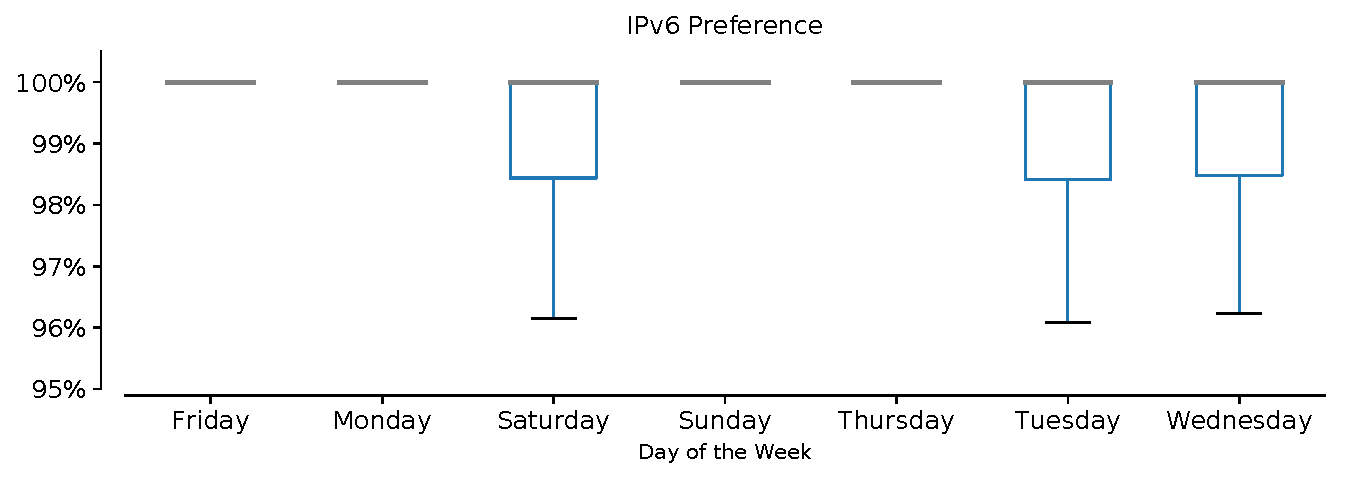
\includegraphics[keepaspectratio, height=4cm, width=15cm]{figures/preference/he-preference-day-boxplot.pdf}
	\caption[IPv6 Preference Boxplot per Day of the Week]{Boxplot shows that IPv6 is preferred around 100\% of the time, but not on Saturdays, Tuesdays, and Wednesdays.}
	\label{fig:IPv6 Preference Daily Boxplot}
\end{figure}
\begin{figure}[!ht]
	\centering
	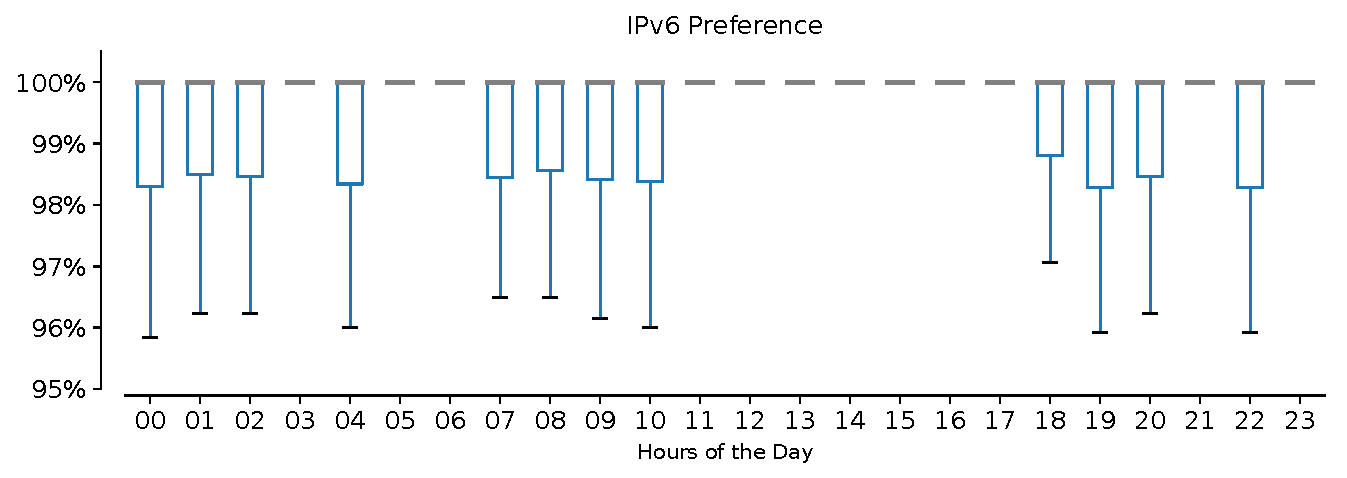
\includegraphics[keepaspectratio, height=4cm, width=15cm]{figures/preference/he-preference-hourly-boxplot.pdf}
	\caption[IPv6 Preference Boxplot per Hours of the Day]{Boxplot shows that TCP connect time over IPv6 is preferred around 100\% during most hours of the day.}
	\label{fig:IPv6 Preference Hourly}
\end{figure}

To get more deeper insights into the TCP connect times over IPv6, we did daily and hourly analysis. For this we first created a new field \textit{days} and got the days of the week from the \textit{dtime} field. 
We performed the steps mentioned before for calculating the IPv6 preference and clustered by \textit{dtime} field. As a result, \cref{IPv6 Preference Daily Boxplot} shows that 
IPv6 is preferred approximately 100\%, but on Saturdays, Tuesday and Wednesday. The reason for this could be that these days are the peak days when users are requesting content 
form Netflix OCA servers. Similarly, the hourly boxplot in \cref{fig:IPv6 Preference Hourly} shows that there are few hours which can be considered peak hours for watching content 
on Netflix as the preference is not 100\% for these hours of the day.

\FloatBarrier
\section{Latency and Delay}\label{chapter:tcppd}
\begin{figure}[!ht]
	\centering
	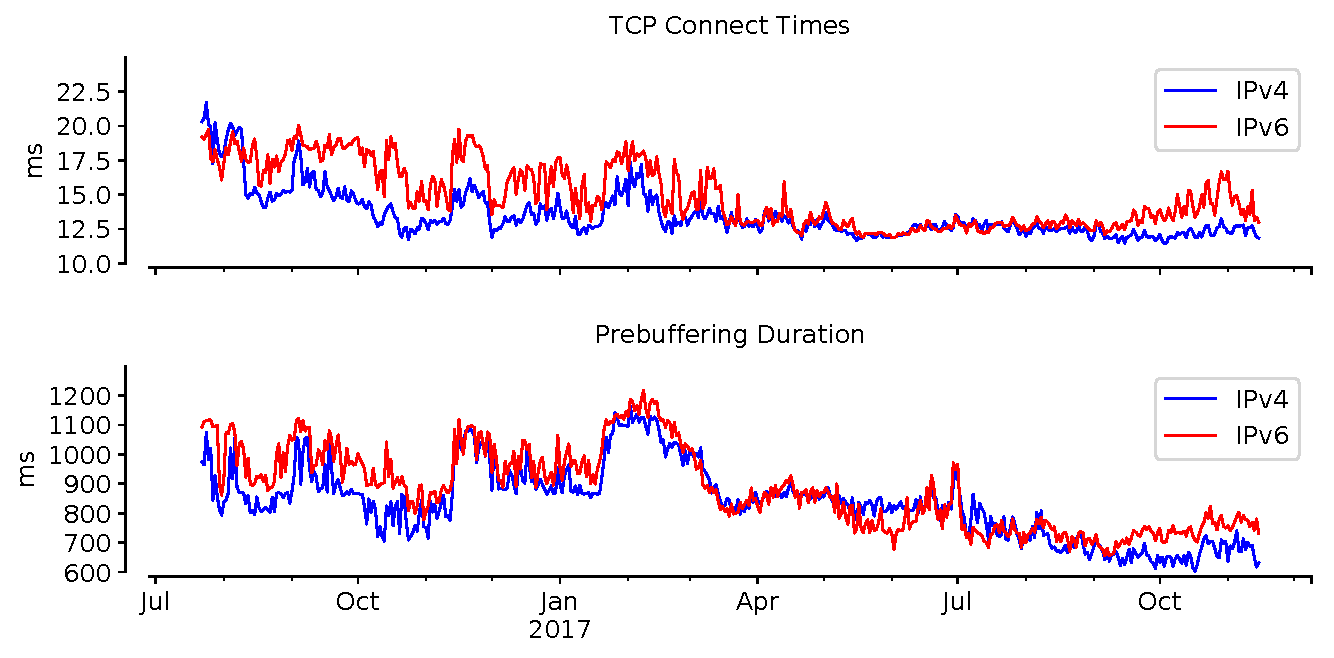
\includegraphics[keepaspectratio, height=5cm, width=15cm]{figures/tcp/netflix-tcp-pd-timeseries-separate.pdf}
	\caption[Connect Time and Prebuffering Duration for IPv4 and IPv6 Timeseries]{Timeseries depicting the TCP connect times (\textit{connect\_time} field) and Prebuffering Duration (\textit{prebuffering\_duration} field) for IPv4 and IPv6. We are applying a median aggregate here and graph resembles similar curves over both the address families.}
	\label{fig:Connect Time and Prebuffering Duration for IPv4 and IPv6 Timeseries}
\end{figure}
\begin{figure}[!ht]
	\centering
	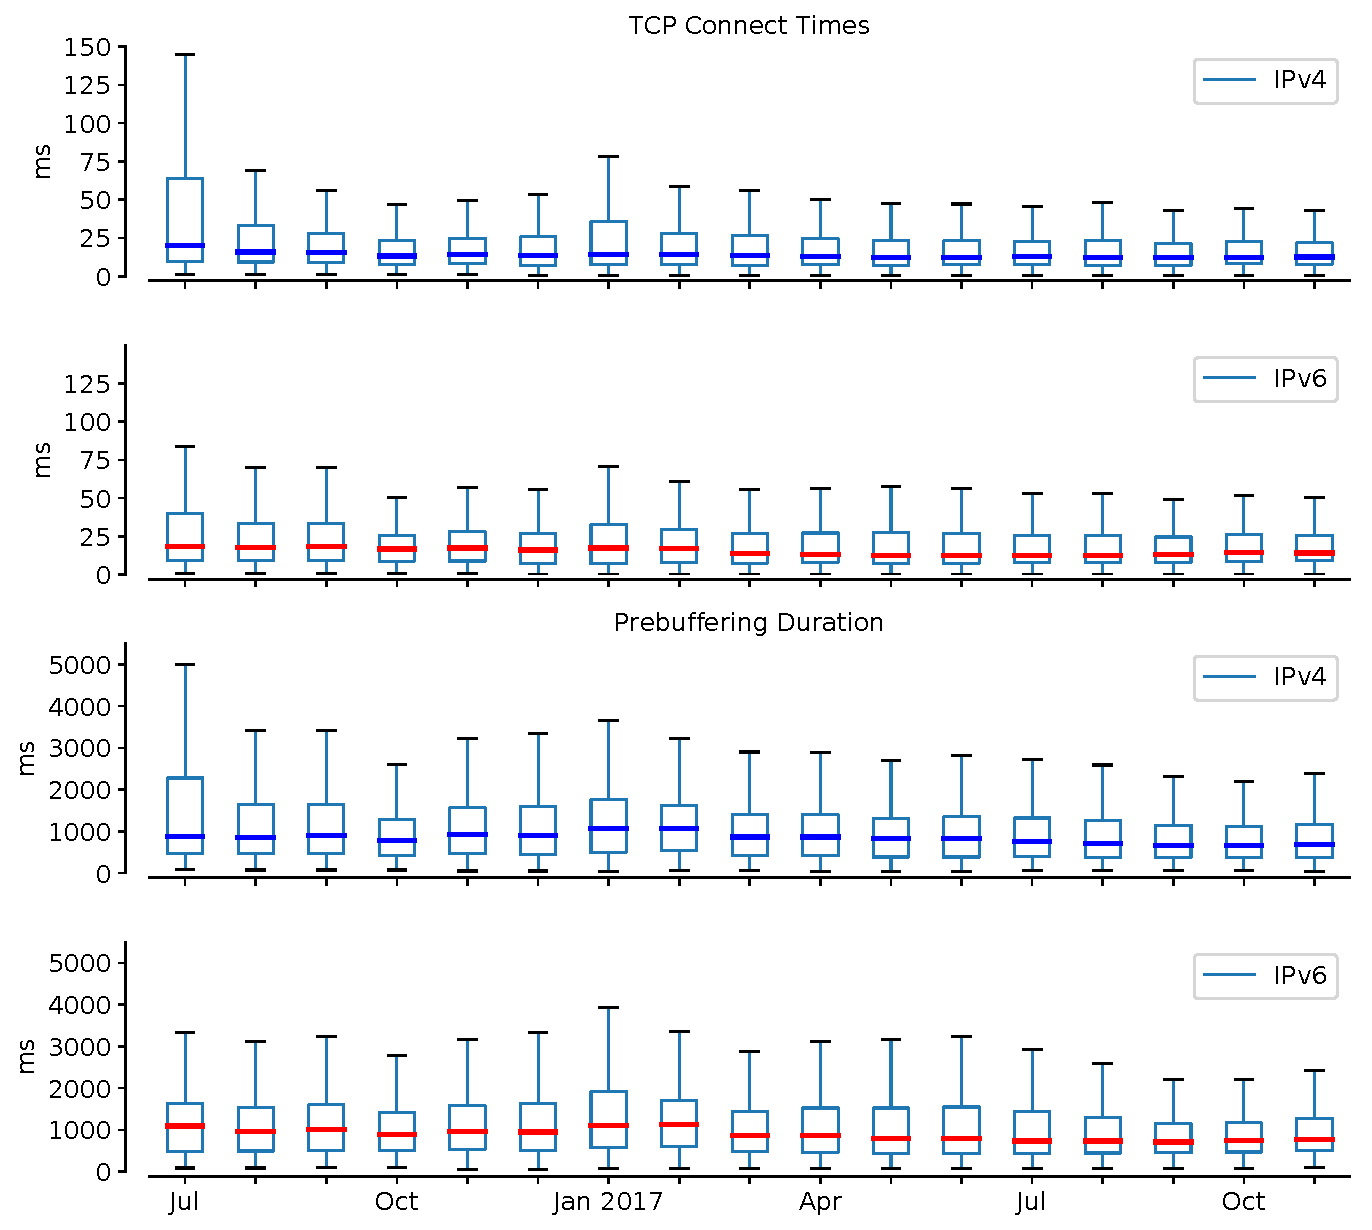
\includegraphics[keepaspectratio, height=8cm, width=15cm]{figures/tcp/netflix-delay-boxplot-separate.pdf}
	\caption[TCP Connect Times and Prebuffering Duration Boxplot Separate]{Boxplot showing the TCP connect times and Prebuffering Duration over both the familys. It resembles the results from the timeseries \cref{fig:Connect Time and Prebuffering Duration for IPv4 and IPv6 Timeseries}.}
	\label{fig:Connect Times and Prebuffering Duration for IPv4 and IPv6 Boxplot}
\end{figure}
After checking the IPv6 preference, we now know that clients prefer streaming videos over IPv6. It would be good to investigate how IPv6 performance compares with IPv4. Here,
we are considering the \textit{connect\_time} and \textit{prebuffering\_duration} fields that are defined in \cref{table:netflix}. We first want to see how TCP connect times and prebuffering durations perform for both the address families.
\cref{fig:Connect Time and Prebuffering Duration for IPv4 and IPv6 Timeseries} shows the timeseries for both the address families, and we have group by \textit{dtime} field and are considering the median aggregate here, so that a single vantage point doesn't bias the results.
As we can see, the graph resembles similar curves for both the Address Family’s. We have converted the connect time and pre-buffering duration to 'ms' to get a better understanding. The median TCP connect times lies between 10-25 ms and the median pre-buffering duration lies between 600-1200 ms for both the address families.
To get more clear view of the delays, we plot the boxplots for both the address familys. We filter the data with respect to the address family i.e. IPv4 or IPv6, and now we can see in the figure \cref{fig:Connect Times and Prebuffering Duration for IPv4 and IPv6 Boxplot} that the graphs resembles the timeseries \cref{fig:Connect Time and Prebuffering Duration for IPv4 and IPv6 Timeseries}.
We further investigate the distribution of delays, here also, we filter the data along IPv4 and IPv6 and then take the CDF of the desired attributes. \cref{fig:Connect Time and Prebuffering Duration CDF for IPv4 and IPv6} shows the CDF of connect times and prebuffering durations. Although it resembles the timeseries and boxplots, but we cannot see
much difference between IPv4 and IPv6 performance. Thus, it would be good to compare the deltas i.e. the difference between the two address family's.

\begin{figure}
	\centering
	\begin{minipage}{0.5\textwidth}
		\centering
		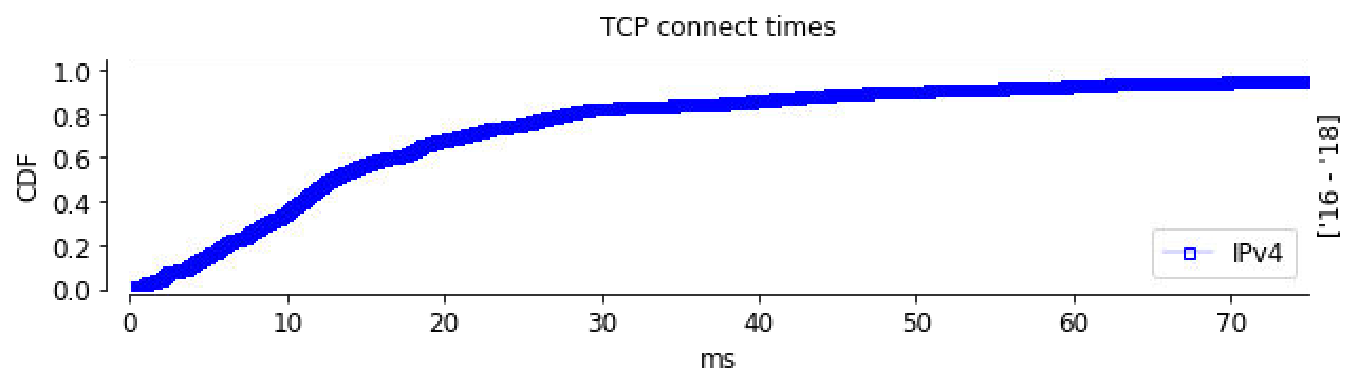
\includegraphics[keepaspectratio, height=5cm, width=8.5cm]{figures/tcp/netflix-syn-time-absolute-difference-v4.pdf}
	\end{minipage}
	\begin{minipage}{0.5\textwidth}
		\centering
		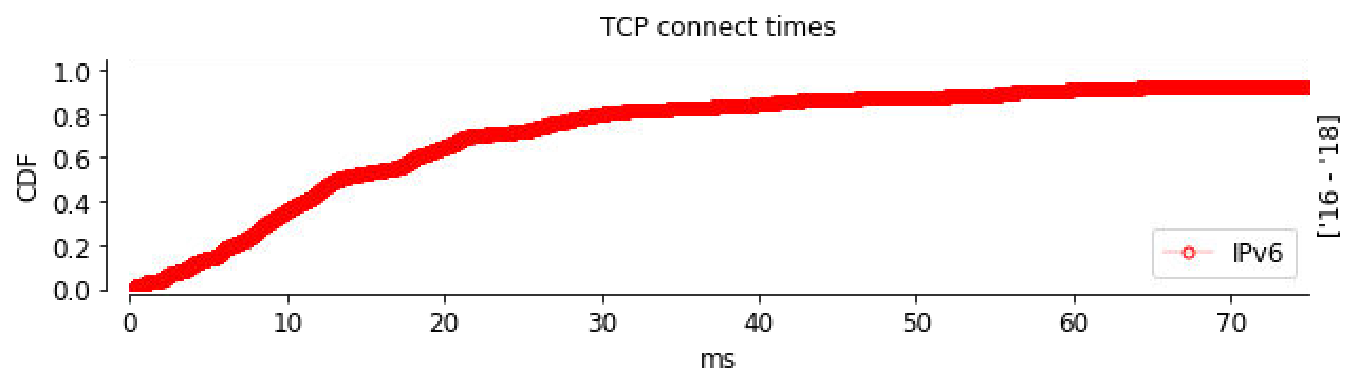
\includegraphics[keepaspectratio, height=5cm, width=8.5cm]{figures/tcp/netflix-syn-time-absolute-difference-v6.pdf}
	\end{minipage}
	\begin{minipage}{0.5\textwidth}
		\centering
		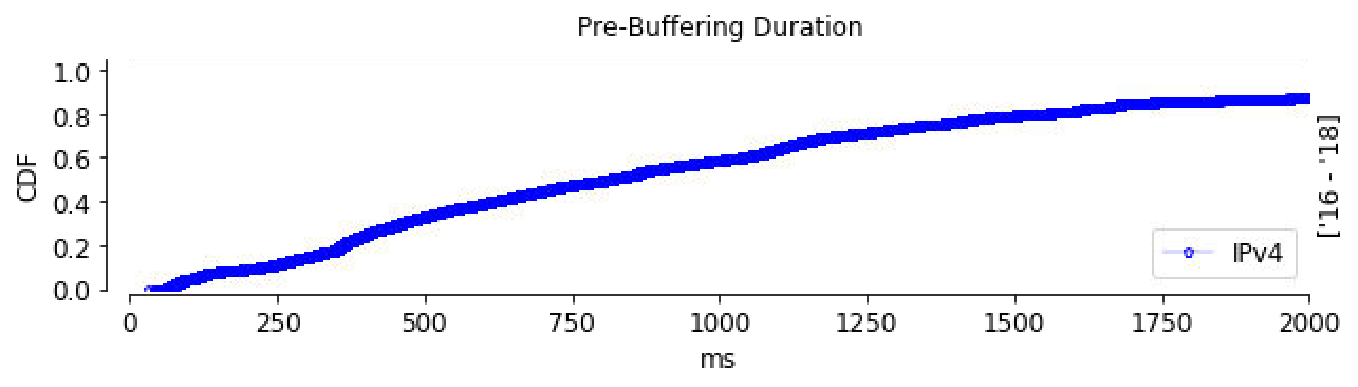
\includegraphics[keepaspectratio, height=5cm, width=8.5cm]{figures/tcp/netflix-prebuffering-duration-absolute-difference-v4.pdf}
	\end{minipage}
	\begin{minipage}{0.5\textwidth}
		\centering
		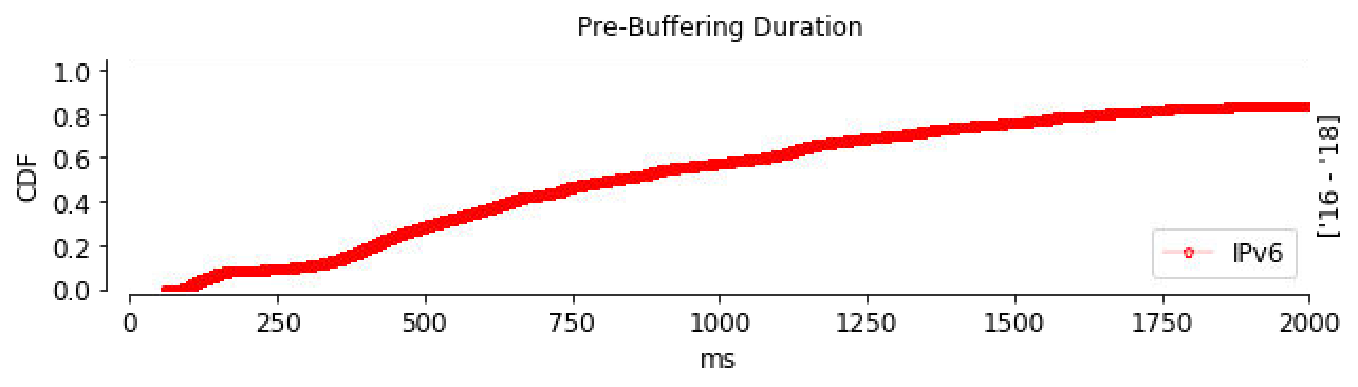
\includegraphics[keepaspectratio, height=5cm, width=8.5cm]{figures/tcp/netflix-prebuffering-duration-absolute-difference-v6.pdf}
	\end{minipage}
	\caption[Connect Time and Prebuffering Duration CDF for IPv4 and IPv6]{CDF of TCP Connect Times and Prebuffering Duration for IPv4 and IPv6. We cannot see much difference between the address family's and it would be good to check the deltas here.}
	\label{fig:Connect Time and Prebuffering Duration CDF for IPv4 and IPv6}
\end{figure}

\subsection*{\textit{Latency and Delay Deltas}}

Let \textit{tc(y)} be the time taken to establish a TCP connection over IPv6 to a Netflix video and \textit{tc(x)} be the time taken to establish a TCP connection over IPv4 to the same video.
Similarly, \textit{p(y)} be the prebuffering duration over IPv6 and \textit{p(x)} be the prebuffering duration over IPv4 for accessing a Netflix video.
Also, as already discussed in \cref{chapter:Datasets}, prebuffering duration takes into account DNS resolution times and TCP connect times.
A user desires to get lower latency which can be achived through lower TCP connect times and lower prebuffering duration. To calculate latency over IPv4 and IPv6, we use the
\ref{eq:deltas}, where $\Delta$tc, and $\Delta$p are the differences in TCP connect times and Prebuffering duration respectively.
\begin{equation}\label{eq:deltas}
$$ $\Delta$tc = tc(x) - tc(y)$$
$$ $\Delta$p = p(x) - p(y)$$
\end{equation}

To plot the deltas, we followed the same analysis \cite{bajpaimeasuring} did. To plot the timeseries for this deltas, we calculate the median aggregate on the TCP connect times and the prebuffering duration across all probes on each day.
\cref{fig:TCP Connect Times and Prebuffering Duration Timeseries} shows the timeseries of median TCP connect times and prebuffering duration over IPv4 and IPv6 across all probes.
Here, it can be seen that the TCP connect times were initially higher for IPv4, but eventually decreased with time and remained consistent. Even though IPv6 tend to have higher TCP connect times,
 and only around 0.2 ms slower than IPv4, it plays very important role for the HE algorithm \cite{rfc6555}, as this the stage where HE algorithm decides on the address family which will be used for streaming the video.
As the difference between IPv4 and IPv6 is less than 300ms, therefore IPv6 is preferred most of the time. Also, IPv6 has higher prebuffering durations (around 40ms or more).
For boxplots in \cref{fig:TCP Connect Times and Prebuffering Duration Boxplot}, we have rounded the time to the nearest month. Here, we can see that the median resembles the time series \cref{fig:TCP Connect Times and Prebuffering Duration Timeseries}.
To get more vivid analysis, \cref{fig:TCP connect times and Prebuffering Duration CDF} shows us the distribution of difference in TCP connect times and prebuffering duration for the whole dataset.
For calculating the CDF, we calcualted the deltas and then plotted their CDF. To compare the performance of IPv6 and IPv4, 
we are measuring the TCP connect times to the Netflix OCA (Open Connect Appliances) server, the distribution here shows that 57\% of the connections are slower over IPv6 , with 13\% of them at least 
10 ms slower. For prebuffering duration which is the time to fetch 2 seconds of video at the specified bitrate from the Netflix OCA (Open Connect Appliances) server, the distribution shows that 69\% of the connections are slower over IPv6.

\begin{figure}[!ht]
	\centering
	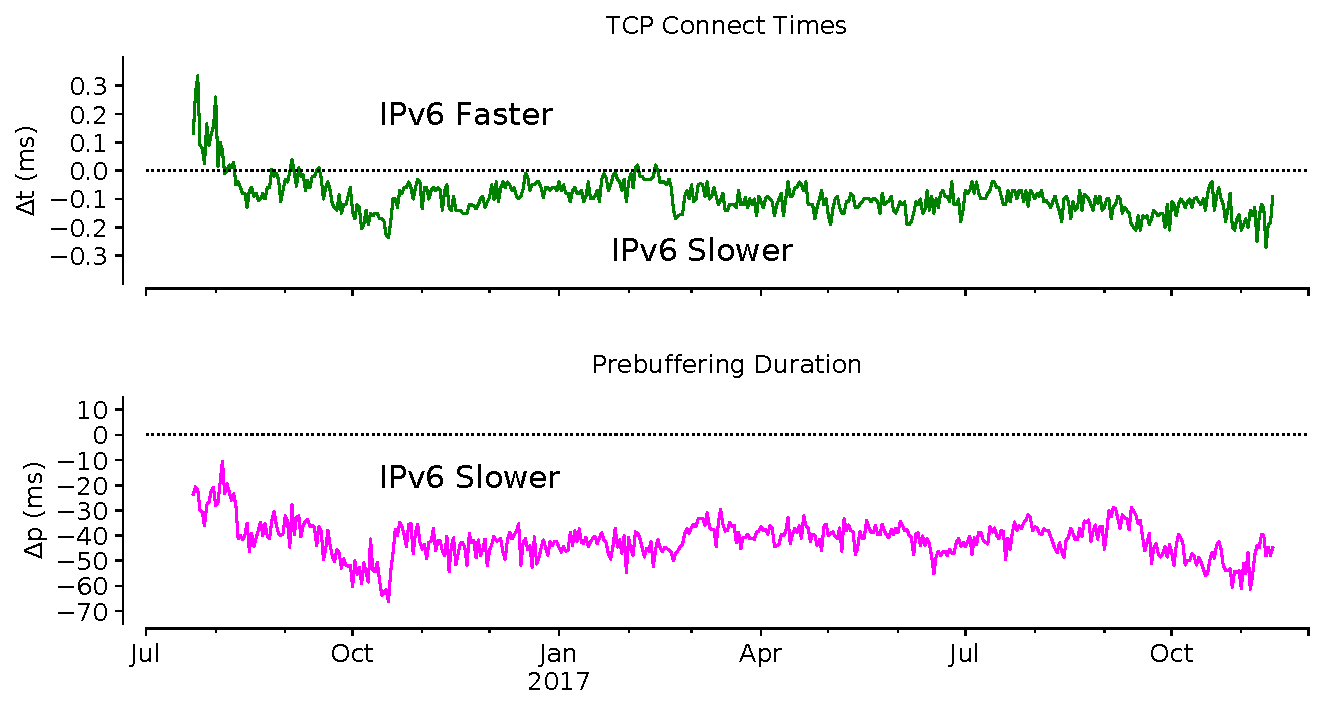
\includegraphics[keepaspectratio, height=5cm, width=15cm]{figures/tcp/netflix-delay-timeseries.pdf}
	\caption[TCP Connect Times and Prebuffering Duration Timeseries]{Time series of difference for TCP connect times and prebuffering durations over IPv4 and IPv6 to Netflix. Latency of around 0.2 ms and higher prebuffering durations (aroun40 ms or more) are observed over IPv6.}
	\label{fig:TCP Connect Times and Prebuffering Duration Timeseries}
\end{figure}
\begin{figure}[!ht]
	\centering
	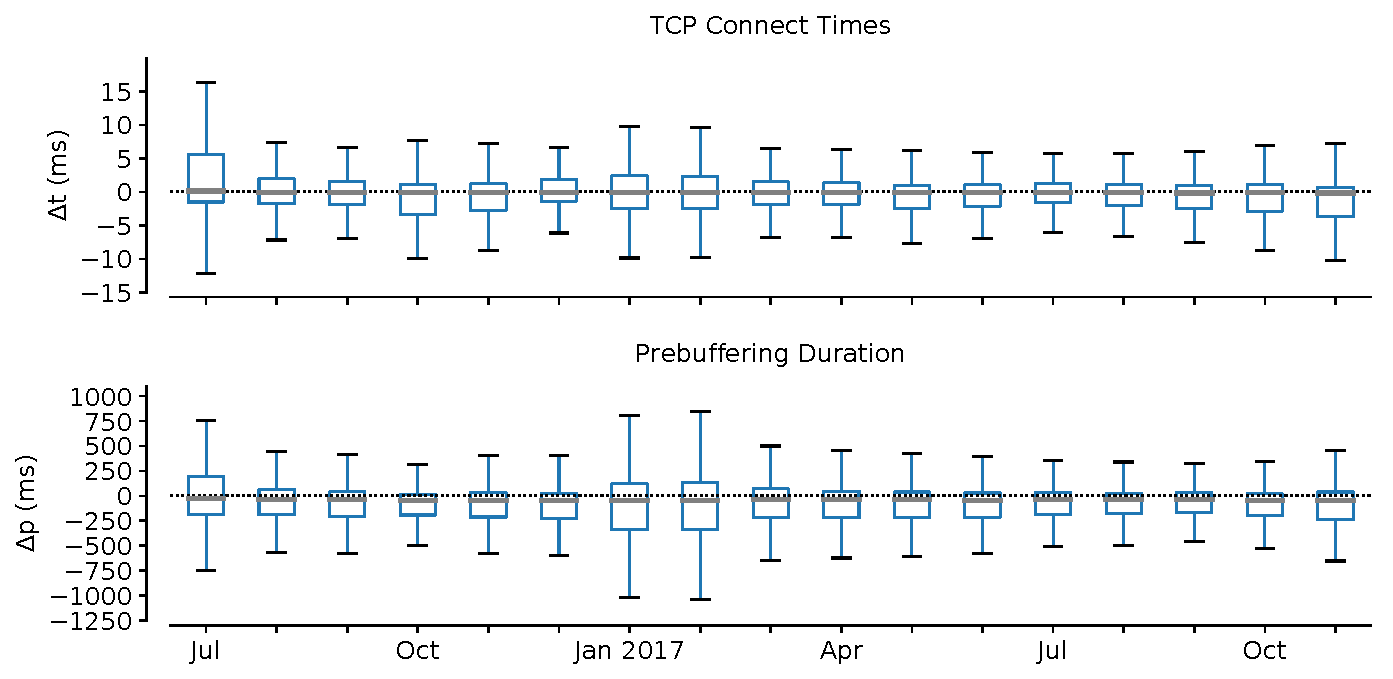
\includegraphics[keepaspectratio, height=5cm, width=15cm]{figures/tcp/netflix-delay-boxplot.pdf}
	\caption[TCP Connect Times and Prebuffering Duration Boxplot]{Boxplots depicting the difference for TCP connect times and prebuffering duration. The median line here resembles the time series \cref{fig:TCP Connect Times and Prebuffering Duration Timeseries}.}
	\label{fig:TCP Connect Times and Prebuffering Duration Boxplot}
\end{figure}

\begin{figure}
	\begin{minipage}{0.6\linewidth}
		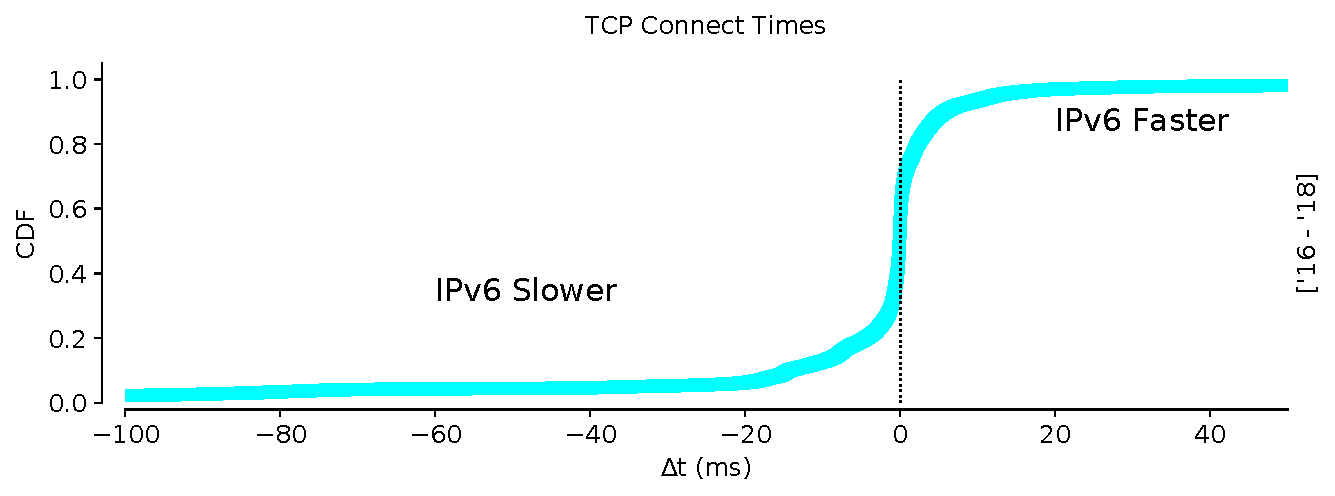
\includegraphics[keepaspectratio, height=2.5cm, width=15cm]{figures/tcp/netflix-syn-time-absolute-difference.pdf}
	\end{minipage}
	\begin{minipage}{0.6\linewidth}
		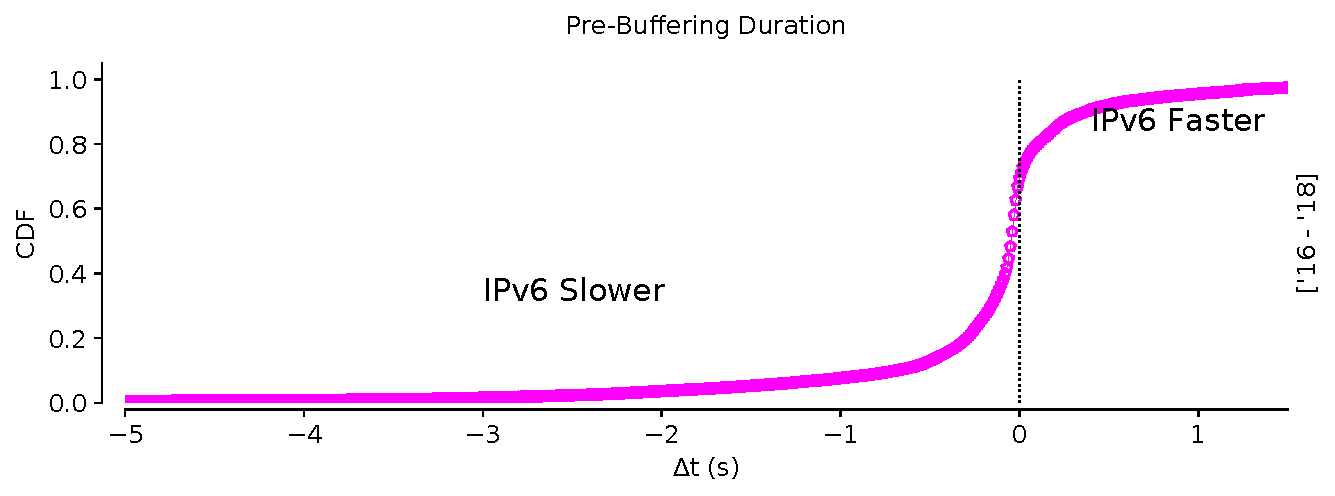
\includegraphics[keepaspectratio, height=2.5cm, width=15cm]{figures/tcp/netflix-prebuffering-duration-absolute-difference.pdf}
	\end{minipage}
\caption[TCP connect times and Prebuffering Duration CDF]{CDF of difference of TCP connect times and Prebuffering Durations for IPv4 and IPv6. The distribution here shows that 57\% of the connections are slower over IPv6 , with 13\% of them at least 
10 ms slower. The prebuffering duration distribution shows that 69\% of the connections are slower over IPv6.}
\label{fig:TCP connect times and Prebuffering Duration CDF}
\end{figure} 

\subsection*{\textit{SKY UK Latency and Delays}}

We wanted to know how Netflix OCA performs compared to when the content server is in an Internet Service Provider (ISP). We already discussed in chapter \ref{chapter:Related Work} about the Open Connect Appliances, Netflix normally places them 
on the Internet Exchange Points (IXPs). We wanted to find out how these OCAs performs compares to when the content is served from an ISP server. Netflix may be saving a lot of capital from placing OCAs at IXPs but are they compromising on the performance.
\cref{fig:TCP Connect Times and Prebuffering Duration Boxplot for BSKYB} gives us a boxplot of TCP connect times and prebuffering duration for Sky UK Limited.
Here, we considered both the probe and the \textit{target} from the same Autonomous System (AS) i.e. "BSKYB-BROADBAND-AS - Sky UK Limited", compared to the rest of the cases.
As can be seen, \cref{fig:TCP Connect Times and Prebuffering Duration Boxplot for BSKYB}, the performance is pretty good when both the user and the \textit{target} belongs to the same AS.

\begin{figure}[!ht]
	\centering
	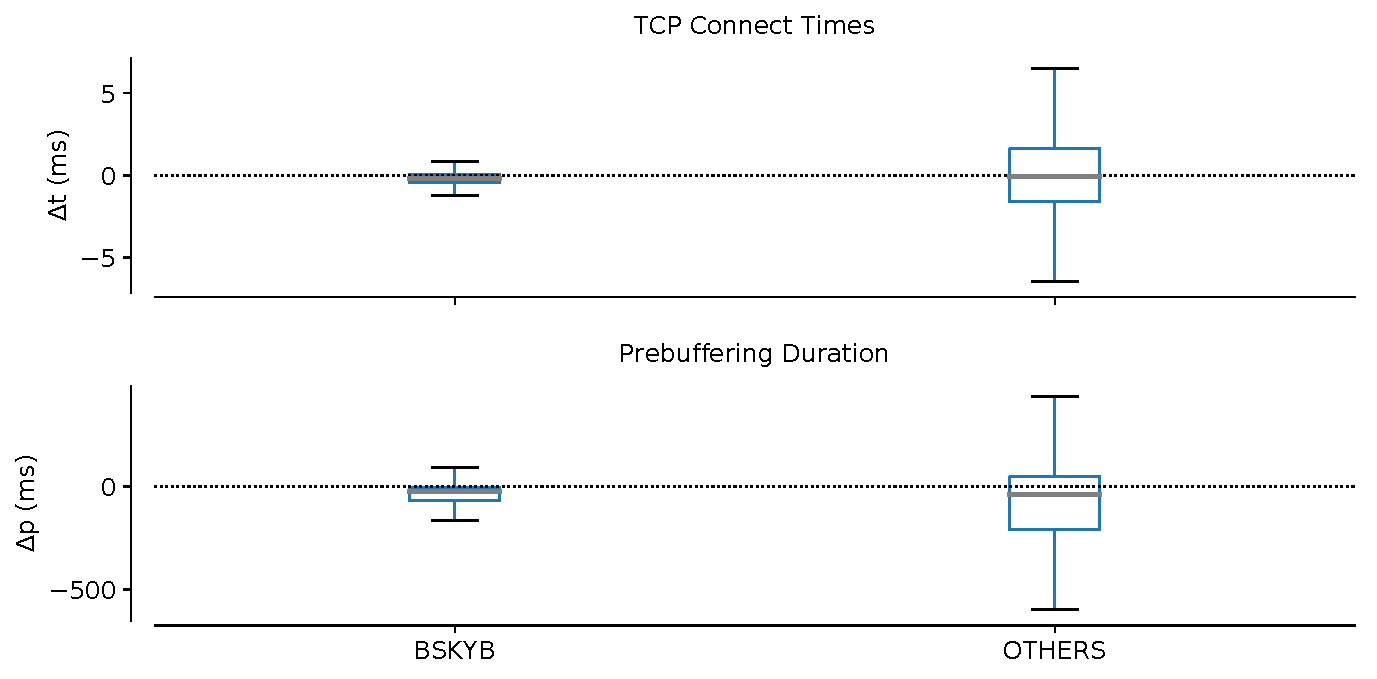
\includegraphics[keepaspectratio, height=4cm, width=15cm]{figures/tcp/netflix-delay-boxplot-bskyb.pdf}
	\caption[TCP Connect Times and Prebuffering Duration Boxplot for BSKYB]{Boxplot for TCP connect times and prebuffering duration for Sky UK Limited. We are comparing the case where both the probe and the \textit{target} belongs to the "BSKYB-BROADBAND-AS - Sky UK Limited" AS compared to the rest of the cases. The performance over BSKYB is good compared to when the probe and \textit{target} are in different ASes.}
	\label{fig:TCP Connect Times and Prebuffering Duration Boxplot for BSKYB}
\end{figure}

\FloatBarrier

\section{Throughput}

\begin{figure}[!ht]
	\centering
	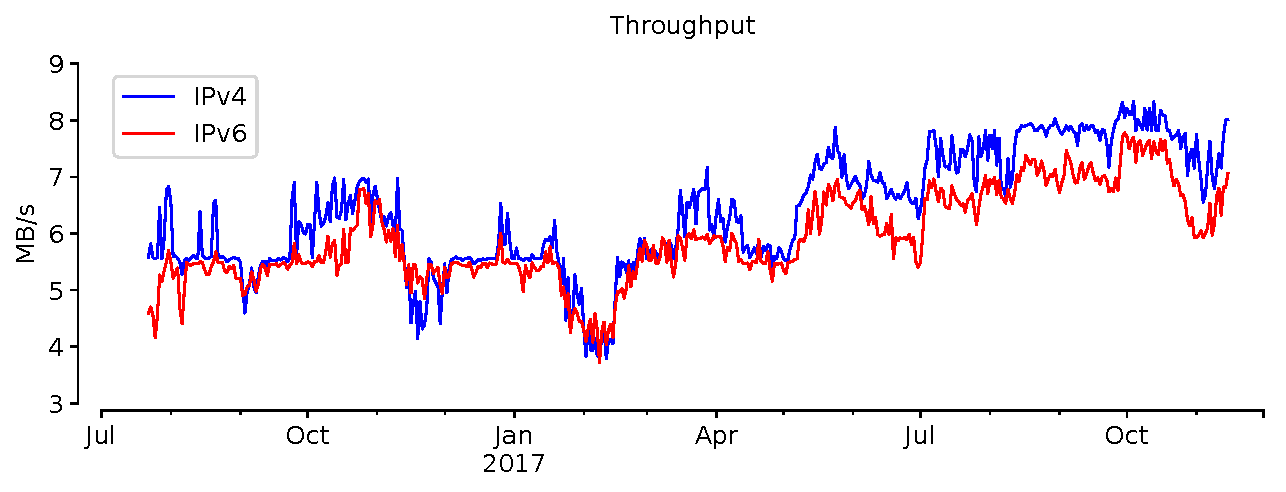
\includegraphics[keepaspectratio, height=4cm, width=15cm]{figures/throughput/netflix-throughput-timeseries-separate.pdf}
	\caption[Throughput Timeseries for IPv4 and Ipv6]{Time series of Throughput for individual address family's i.e. IPv4 and IPv6. We are considering the \textit{bytes\_sec} field described in \cref{table:netflix}. Both the families shows similar curves with throughput between 3-9 MB/s.}
	\label{fig:Throughput Timeseries for IPv4 and Ipv6}
\end{figure}
\begin{figure}[!ht]
	\centering
	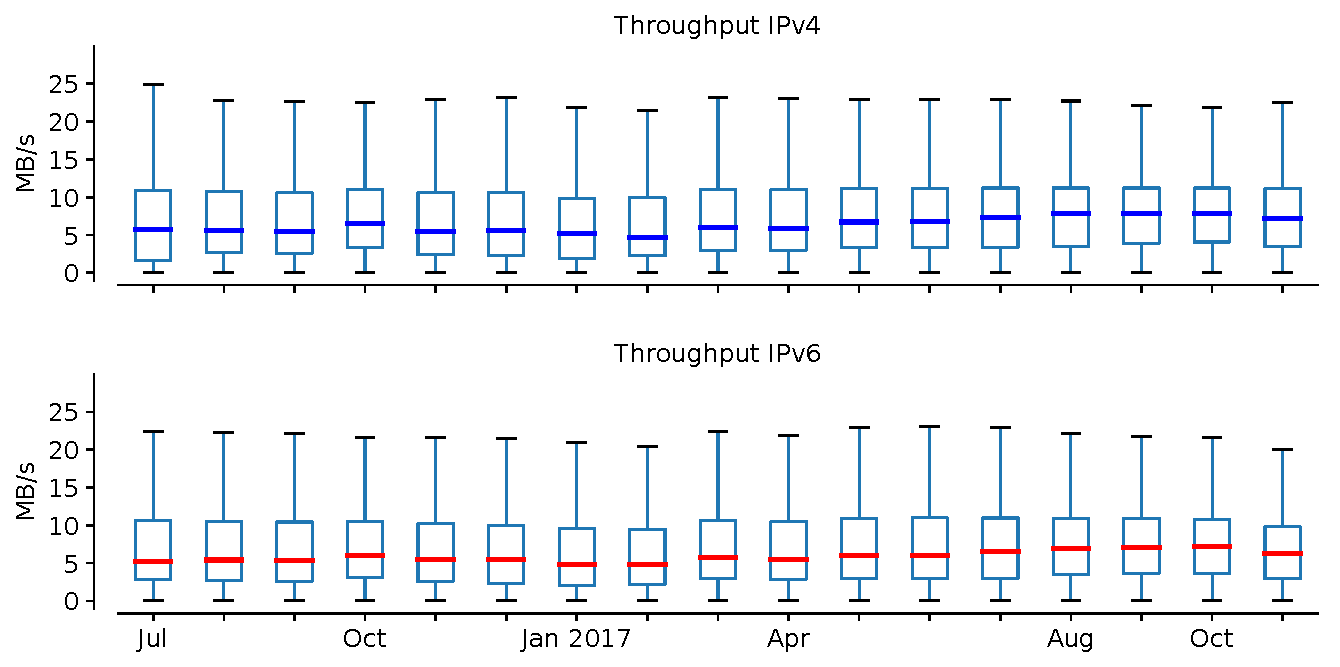
\includegraphics[keepaspectratio, height=5cm, width=15cm]{figures/throughput/netflix-throughput-boxplot-separate.pdf}
	\caption[Throughput Boxplot for IPv4 and IPv6]{Boxplot of throughput over IPv4 and IPv6. We can see the monthly variation here, also the median line resembles the time series in \cref{fig:Throughput Timeseries for IPv4 and Ipv6}.}
	\label{fig:Throughput Boxplot for IPv4 and IPv6}
\end{figure}

After going through \cref{chapter:ipv6preference} we know that clients prefer to stream videos on Netflix over IPv6. We also saw in \cref{chapter:tcppd} that the clients take consistently higher TCP connect times and prebuffering durations
(40ms or more) when compared to IPv4 (see \cref{fig:TCP Connect Times and Prebuffering Duration Timeseries}. To compare their performance, one important factor is achieved throughput, we will now look into this factor and compares the performance over both families.
We first look into the individual performance of IPv4 and IPv6 and then will look into their deltas. \cref{fig:Throughput Timeseries for IPv4 and Ipv6} gives the time series for
both the address families, it shows that both the address families shows similar curves and that the throughput is increasing with time.
We are considering the \textit{bytes\_sec} field from the Netflix \cref{table:netflix.}, and we are taking the median aggregate across
all probes on each day. Also, the throughput for IPv4 and IPv6 lies lies between 3-9 MB/s. To get more deeper insights
we also did the boxplot for IPv4 and IPv6 throughput, and as can be seen in \cref{fig:Throughput Boxplot for IPv4 and IPv6} the monthly
throughput variation over IPv4 and IPv6. The median line resembles the time series in \cref{fig:Throughput Timeseries for IPv4 and Ipv6}. We have 
converted the \textit{bytes\_sec} field into MB/s to get a more realistic view. \cref{fig:Throughput CDF over IPv4 and IPv6} shows the CDF of
throughput over IPv4 and IPv6. We followed the same steps here,
and plotted the CDF of \textit{bytes\_sec} field. The CDF for individual shows similar curves and does not give a clear difference
in the performance of IPv4 and IPv6. 
We need to look into the deltas to see which address family performs better than the other.
 
\begin{figure}[!ht]
	\centering
	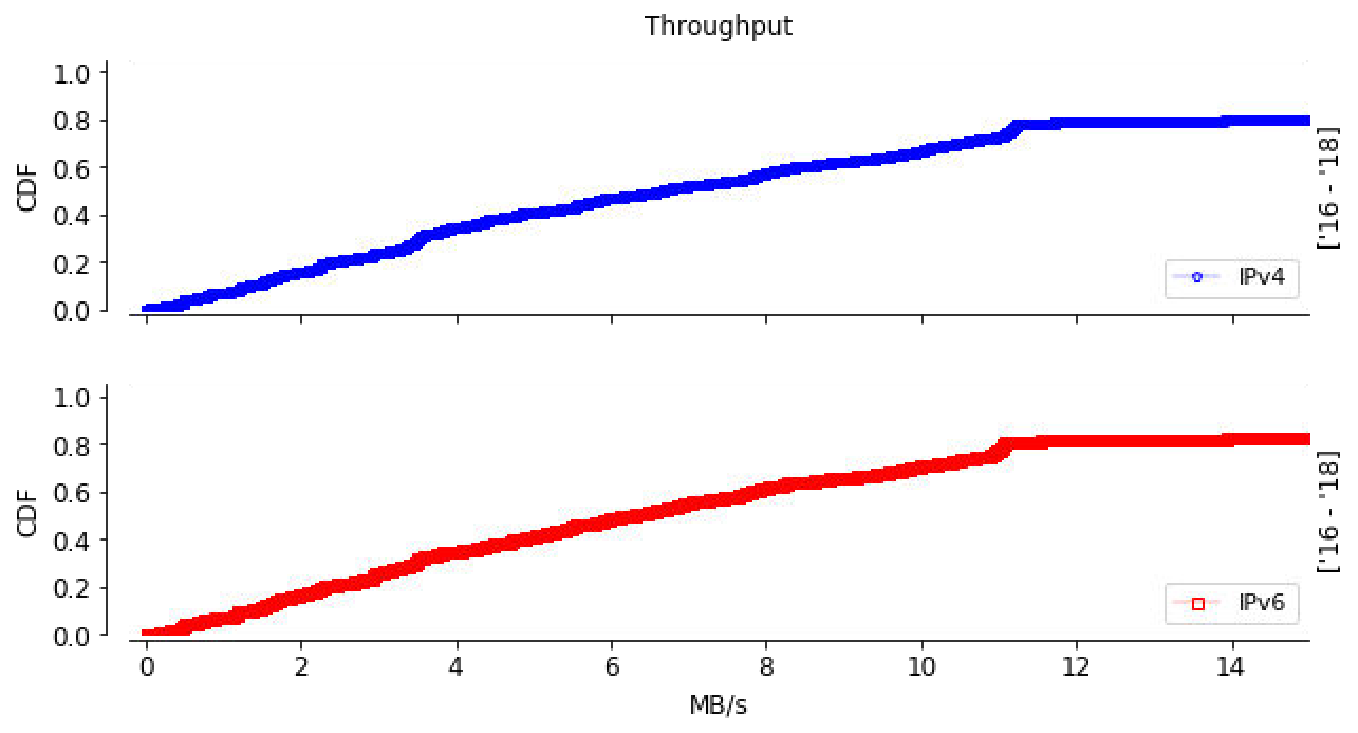
\includegraphics[keepaspectratio, height=5cm, width=15cm]{figures/throughput/netflix-throughput-difference-separate.pdf}
	\caption[Throughput CDF over IPv4 and IPv6]{CDF of throughput over IPv4 and IPv6, shows the similar curves over both the family's. We cannot see much difference in the performance here and thus would be good to plot the CDF for the difference betweent he two families.}
	\label{fig:Throughput CDF over IPv4 and IPv6}
\end{figure}
\FloatBarrier

\subsection*{\textit{Throughput Deltas}}

\begin{figure}[!ht]
	\centering
	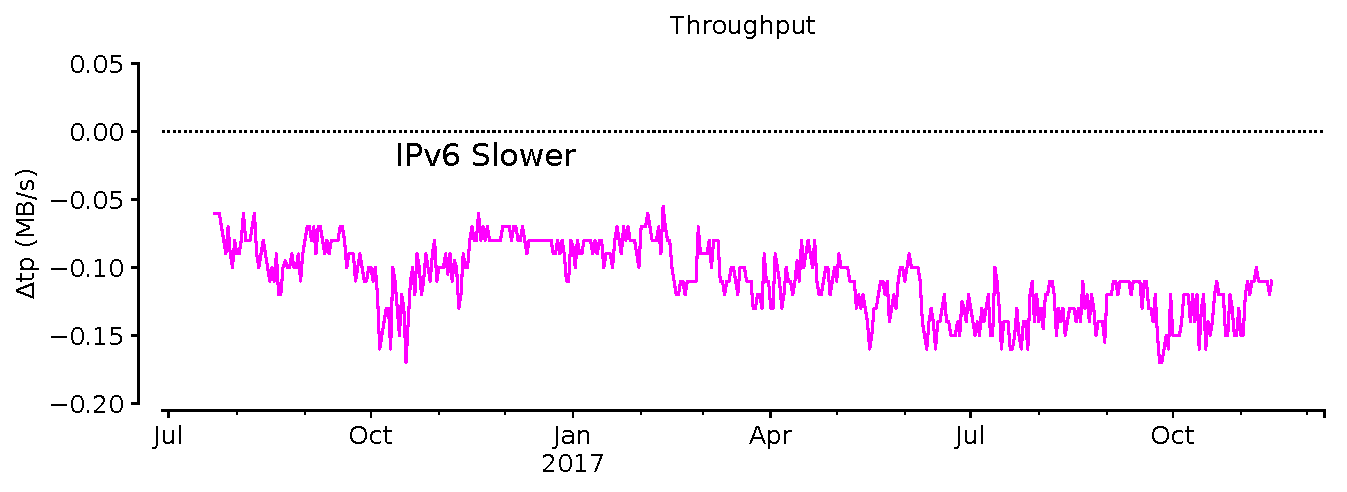
\includegraphics[keepaspectratio, height=4cm, width=15cm]{figures/throughput/netflix-throughput-timeseries.pdf}
	\caption[Throughput Timeseries]{Time series of difference of throughput over IPv4 and IPv6. We plot the median aggregate across all probes on each day. The achieved throughput is consistently lower over Ipv6.}
	\label{fig:Throughput Timeseries}
\end{figure}

\begin{figure}[!ht]
	\centering
	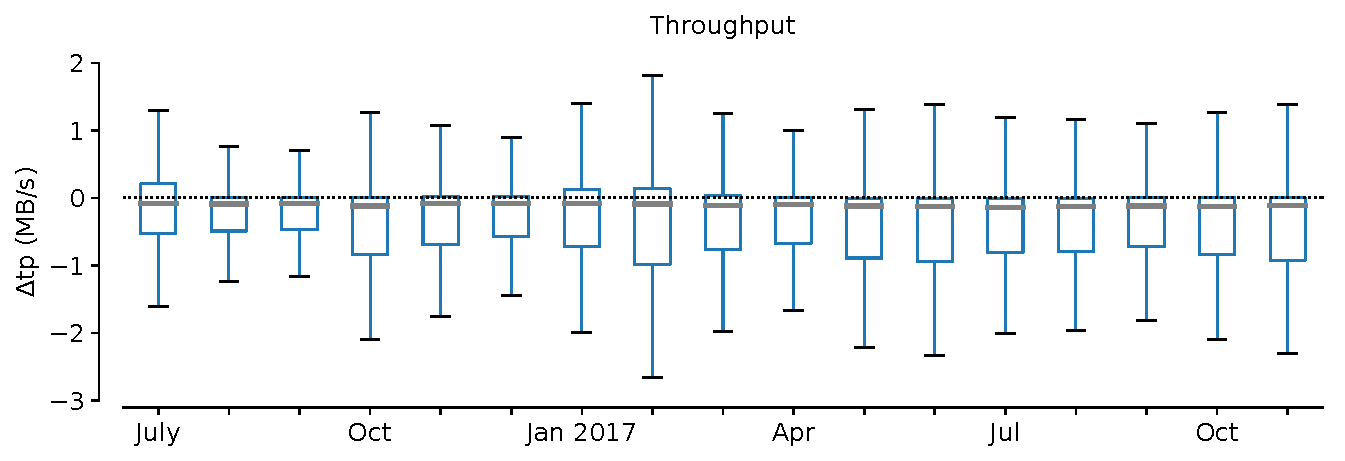
\includegraphics[keepaspectratio, height=4cm, width=15cm]{figures/throughput/netflix-throughput-boxplot.pdf}
	\caption[Throughput Boxplot]{Boxplot of difference of Throughput over IPv4 and IPv6. The figure also shows similar results as the time series \cref{fig:Throughput Timeseries}, depicting lower throughput over IPv6.}
	\label{fig:Throughput Boxplot}
\end{figure}

Before starting with the deltas, we would live to define the terminologies we used to get the results. We are considering the \textit{bytes\_sec} field only and using the same terminilogy \cite{bajpaimeasuring} used. We denote the throughput 
over IPv6 as \textit{tp(y}) and throughput over IPv4 as \textit{tp(x)}. We will use \cref{eq:tpdelatas} where $\Delta$tp is the difference in achieved throughput over both the address families.
To plot the deltas, we first start with the time series, and \cref{fig:Throughput Timeseries} shows us the time series of median aggregae of throughput across all probes over each day.
We can see that the difference is consistent over time and is lower for IPv6 over the whole duration. The negative value indicates a lower throughput over IPv6, also the difference liew between 0-0.2 MB/s.
\cref{fig:Throughput Boxplot} shows the boxplot of difference of throughput over IPv4 and IPv6. The median line shows similar curves as the time series \cref{fig:Throughput Timeseries}, depicting lower throughput over IPv6.
To get a more clear picture about the performance, we plot the CDF of \textit{bytes\_sec} field. For CDF, we first compute the difference of throughput over IPv6 and IPv4 and then take the CDf of that difference.
\cref{fig:Throughput CDF} shows the CDF of difference of throughput over IPv4 and IPv6. Around 73% of the times, IPv6 achieved lower throughput. \cite{bajpaimeasuring} informs us when a stall event is triggered, the test steps down
to a lower resolution video. This subsequently lowers the achieved throughput because th test the drops to the next highest bitrate and begin downloading from the start again. This enables the highest resolution
bitrate streaming over a connection without any disruptions. Vaibhav Bajpai et al. in \cite{bajpaimeasuring} further informs us that the test maintains a playout buffer and that it should wait before requesting 
any frames till the previous buffer is empty. The playout buffer can store a playable video of 40s only.
\cref{fig:Throughput Boxplot by Days} further investigates the difference in throughput over IPv6 and IPv4 over different days of the week. The throughput over IPv6 is consistently lower on all the days. 
\begin{equation}\label{eq:tpdeltas}
$$ $\Delta$tp = tp(y) - tp(x)$$
\end{equation}

\begin{figure}[!ht]
	\centering
	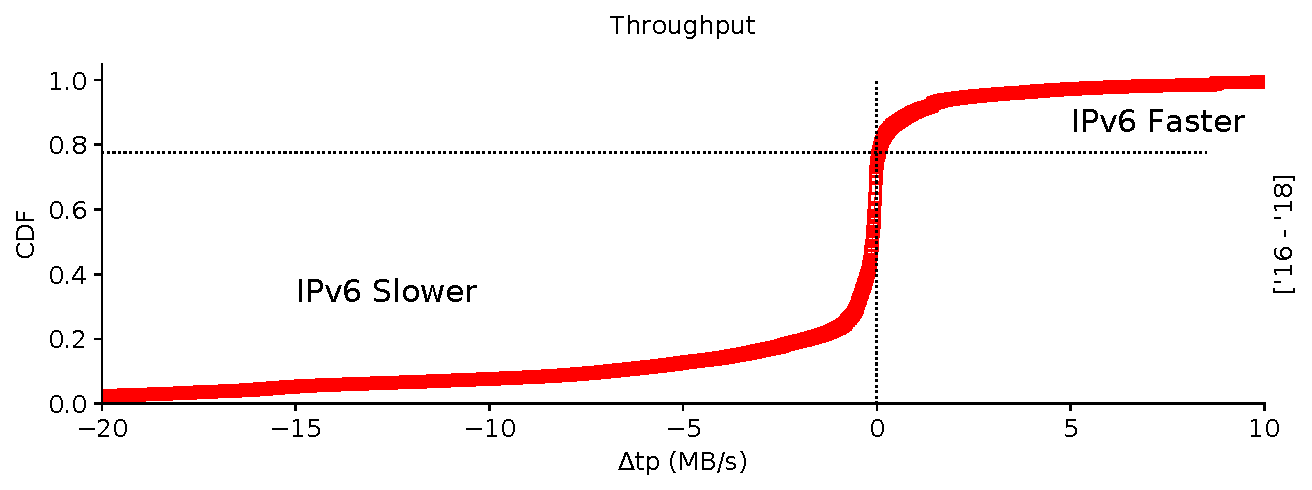
\includegraphics[keepaspectratio, height=4cm, width=15cm]{figures/throughput/netflix-throughput-difference.pdf}
	\caption[Throughput CDF]{CDF shows the distribution of difference of throughput over IPv6 and IPv4. Around 73\% of the times, IPv6 achieved lower throughput.}
	\label{fig:Throughput CDF}
\end{figure} 
\begin{figure}[!ht]
	\centering
	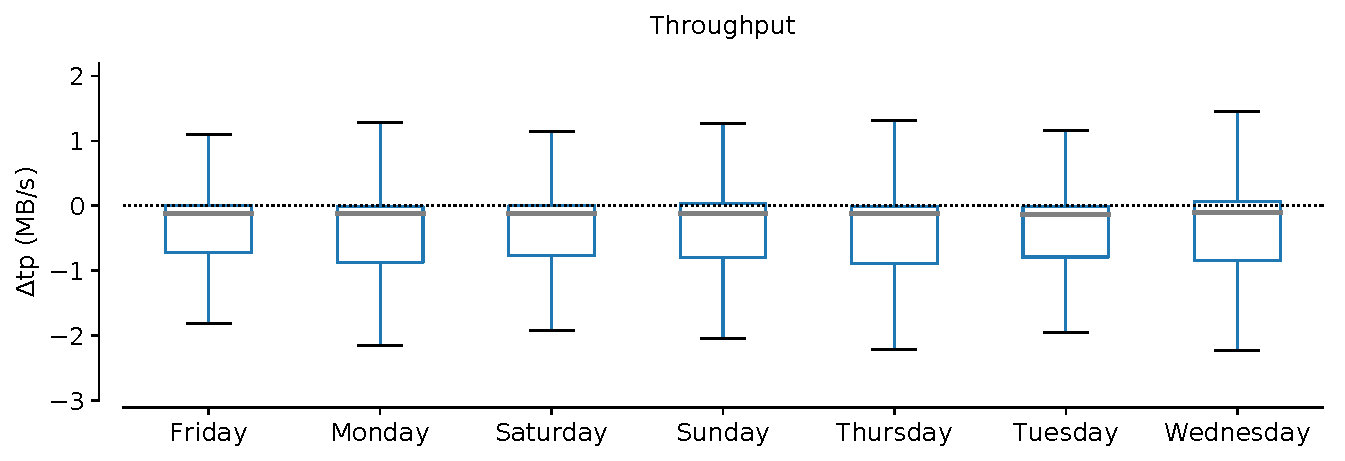
\includegraphics[keepaspectratio, height=4cm, width=15cm]{figures/throughput/netflix-throughput-boxplot-by-days.pdf}
	\caption[Throughput Boxplot by Days]{Boxplot of difference of throughput over IPv6 and IPv4. The throughput is consistently lower over IPv6 on all days of the week.}
	\label{fig:Throughput Boxplot by Days}
\end{figure}

\FloatBarrier

\section{Stall Events}

\begin{figure}[!ht]
	\centering
	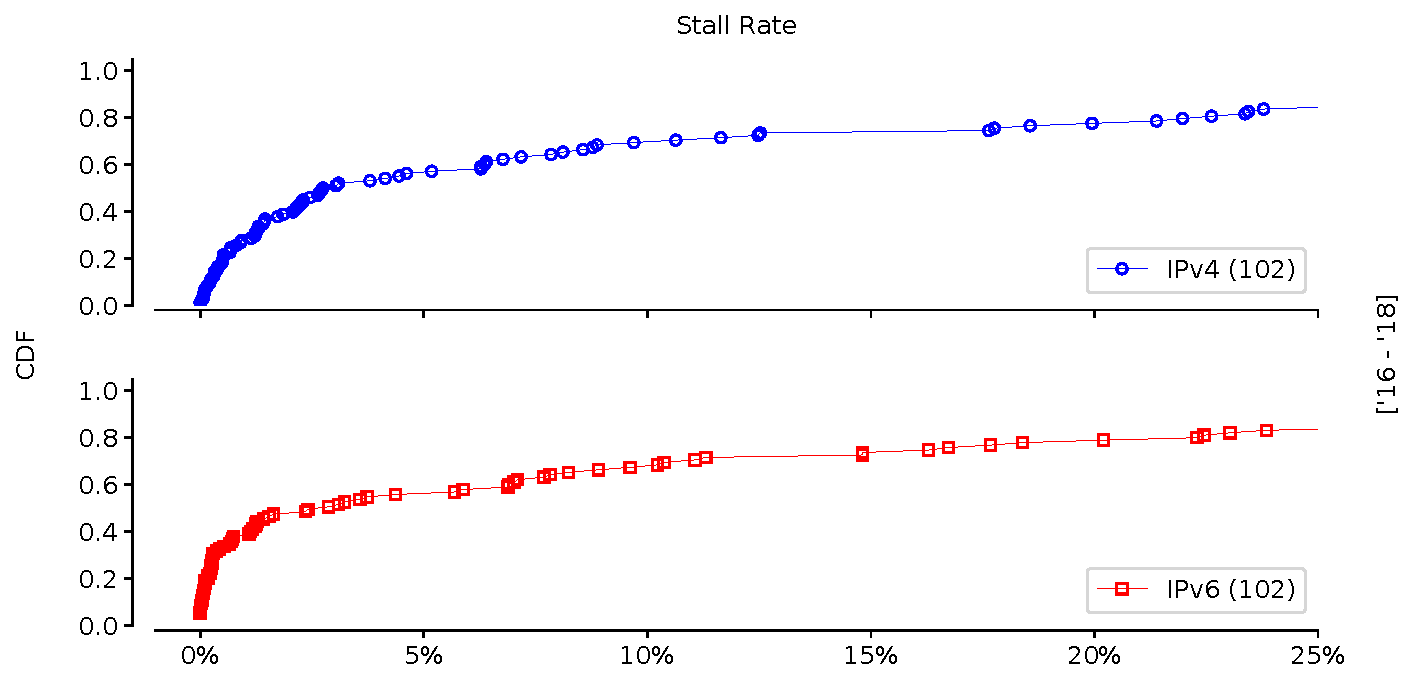
\includegraphics[keepaspectratio, height=5cm, width=15cm]{figures/stall/netflix-stall-rate-probes-cdf.pdf}
	\caption[Stall Rate CDF]{CDF of stall rate over IPv4 and IPv6. 70\% of the probes witness stall rate less than 10\% over both IPv4 and IPv6.}
	\label{fig:Stall Rate CDF}
\end{figure}
We now know that TCP connect times, prebuffering durations and througpput are worse over IPv6. We also know that clients prefer to stream videos over IPv6. 
We now look into stall events and stall durations over IPv4 and IPv6 to see which one performed better. We will look into \textit{stall\_events} and \textit{stall\_duration\_total} field that we already defined in \cref{table:netflix}.
\cite{bajpaimeasuring} defines a stall as an event that occurs during playback in situations when a frame is not recieved during its playout time. 
Throughput constraints leads to stall events which is caused by the bottlenecks between Netflix OCA and the client path. Results from SamKnows speed tests \cite{bajpaipam} are used to ignore unnecessary
stalling, so as to limit maximum bit rate the the client will attempt to download. SamKnows test uses this concept and use the playout buffer of 40s. Thus, incase of a stall event
rebuffering is done before resuming the playout timer \cref{fig:sequencediagram}. To not exceed this playout buffer capacity, media downloads are paced. 
We first define the stall rates over both the address families i.e. Ipv4 and IPv6.  \textit{Stall Rate} is defined as the number of stall events to the total number of iterations of the test \cite{bajpaimeasuring}. 
We are considering the \textit{stall\_event} field here, and after calculating the stal rate we take a CDF of it.
\cref{fig:Stall Rate CDF} depicts the distribution of stall rates over IPv4 and IPv6 across all probes. As can be seen, both the address families shows comparable stall rates. Around 70\% of the probes witness stall rate less than 10\% over both IPv4 and IPv6.
\begin{figure}[!ht]
	\centering
	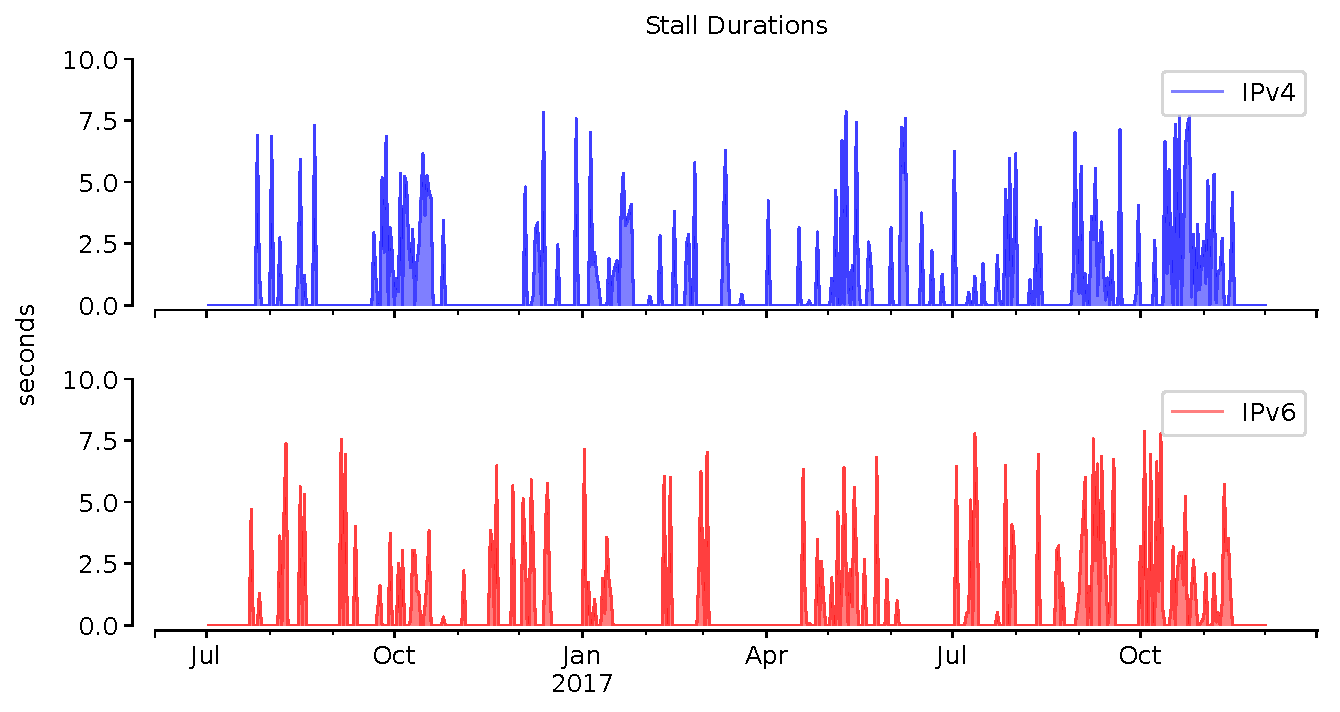
\includegraphics[keepaspectratio, height=5cm, width=15cm]{figures/stall/netflix-stall-durations-timeseries-separate.pdf}
	\caption[Stall Duration Timeseries for IPv4 and IPv6]{Time series of Stall durations over IPv4 and IPv6. We took the median aggregate of \textit{stall\_durations\_total} across all probes on each day. Stall durations have been consistent over time.}
	\label{fig:Stall Duration Timeseries for IPv4 and IPv6}
\end{figure}
\begin{figure}[!ht]
	\centering
	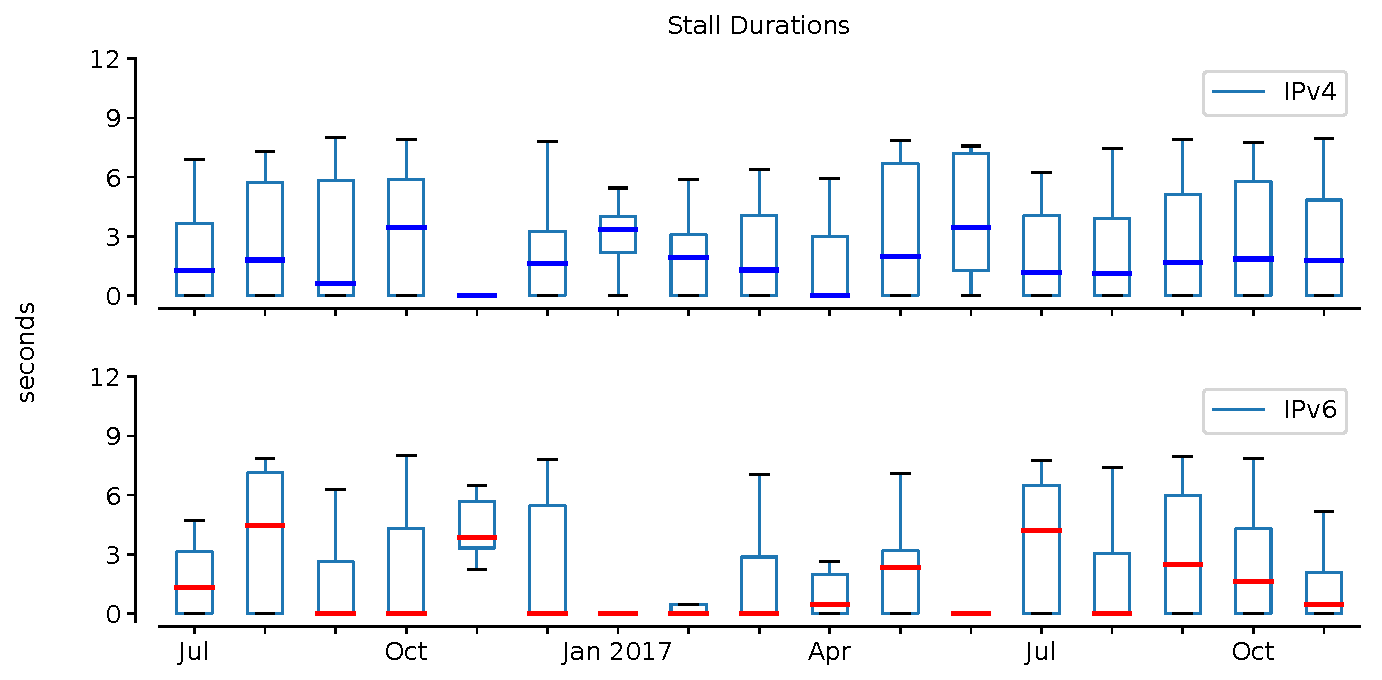
\includegraphics[keepaspectratio, height=5cm, width=15cm]{figures/stall/netflix-stall-durations-boxplot.pdf}
	\caption[Stall Duration Boxplot for IPv4 and IPv6]{Boxplot of Stall durations over IPv4 and IPv6. We have rounded the time to the nearest month, and we are measuring the stall durations over the period. The variation can be seen over different months.}
	\label{fig:Stall Duration Boxplot for IPv4 and IPv6}
\end{figure}
\textit{stall\_durations\_total} field gives us the total durations of stall as already discussed in \cref{table:netflix}. We know measure the stall durations over IPv4 and IPv6. \cref{fig:Stall Duration Timeseries for IPv4 and IPv6}
gives us the time series of stall durations over IPv4 and IPv6. We took the median aggregate of \textit{stall\_durations\_total} across all probes on each day. Stall durations have been consistent over time. To see variation over different months \cref{fig:Stall Duration Boxplot for IPv4 and IPv6}
gives us the boxplot of stall durations variation over different months. 
To get a clear picture \cref{fig:Stall Duration CDF for IPv4 and IPv6} shows us the CDF of stall durations over IPv4 and IPv6. Here, we cannot see much of difference as both the address
families shows similar results. It would be good to check their deltas.
\begin{figure}[!ht]
	\centering
	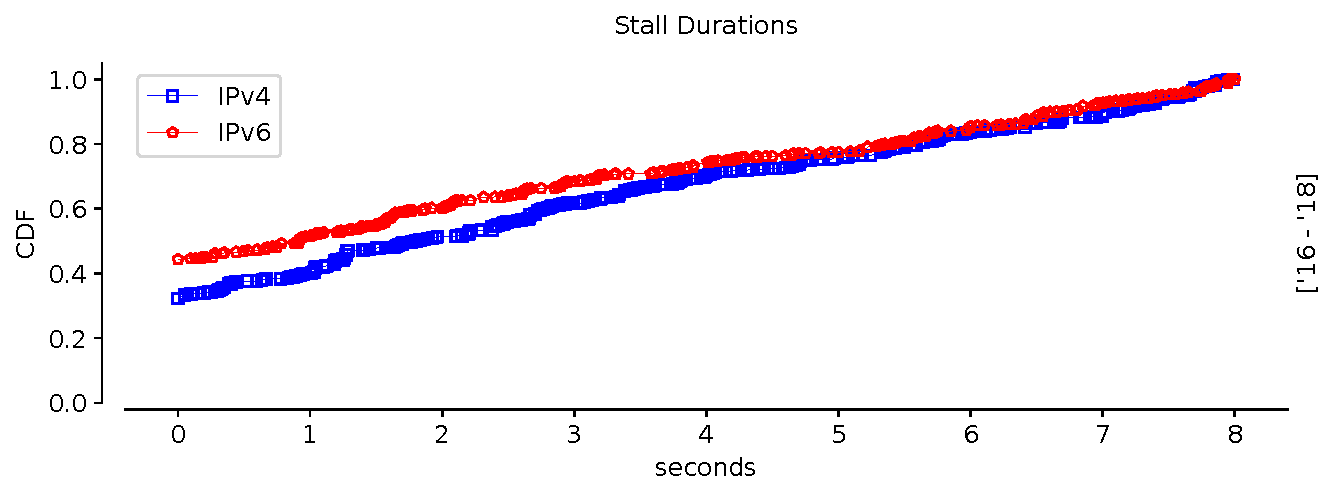
\includegraphics[keepaspectratio, height=4cm, width=15cm]{figures/stall/netflix-stall-durations-absolute-difference-separate-one.pdf}
	\caption[Stall Duration CDF for IPv4 and IPv6]{CDF of stall durations over IPv4 and IPv6. Both the address families shows similar curves.}
	\label{fig:Stall Duration CDF for IPv4 and IPv6}
\end{figure}

\subsection*{\textit{Stall Events Deltas}}

As individual CDFs doesn't give much information, we will calculate the difference of stall durations over IPv4 and IPv6 over both the families. We take the same terminology defined in \cite{bajpaimeasuring}.
We use \cref{eq:stdeltas} to calculate the difference in stall durations over IPv4 and IPv6. Here, $\Delta$st gives the delta for both the address families. \textit{st(y)} is the stall duration over IPv6
and \textit{st(x)} is the stall duration over IPv4. \cref{fig:Stall Duration CDF} gives us the distribution of difference of stall duratiosn over IPv4 and IPv6. Here, we calculated the difference of stalldurations and took a CDF of it.
Positive values indicates that stall durations are lower over IPv6. 41% of the samples experience lower stall durations over IPv4, whereas, 59% of the samples experience lower stall durations over IPv6 with around 25% of them at least 5 seconds shorter.
\cref{fig:Stall Duration Difference Boxplot} shows us boxplot of difference of stall durations over IPv4 and Ipv6. It shows the similar characteristics as in \cref{fig:Stall Duration Boxplot for IPv4 and IPv6} and we can see the variation between different months.
\begin{equation}\label{eq:stdeltas}
$$ $\Delta$st = st(x) - st(y)$$
\end{equation}

\begin{figure}[!ht]
	\centering
	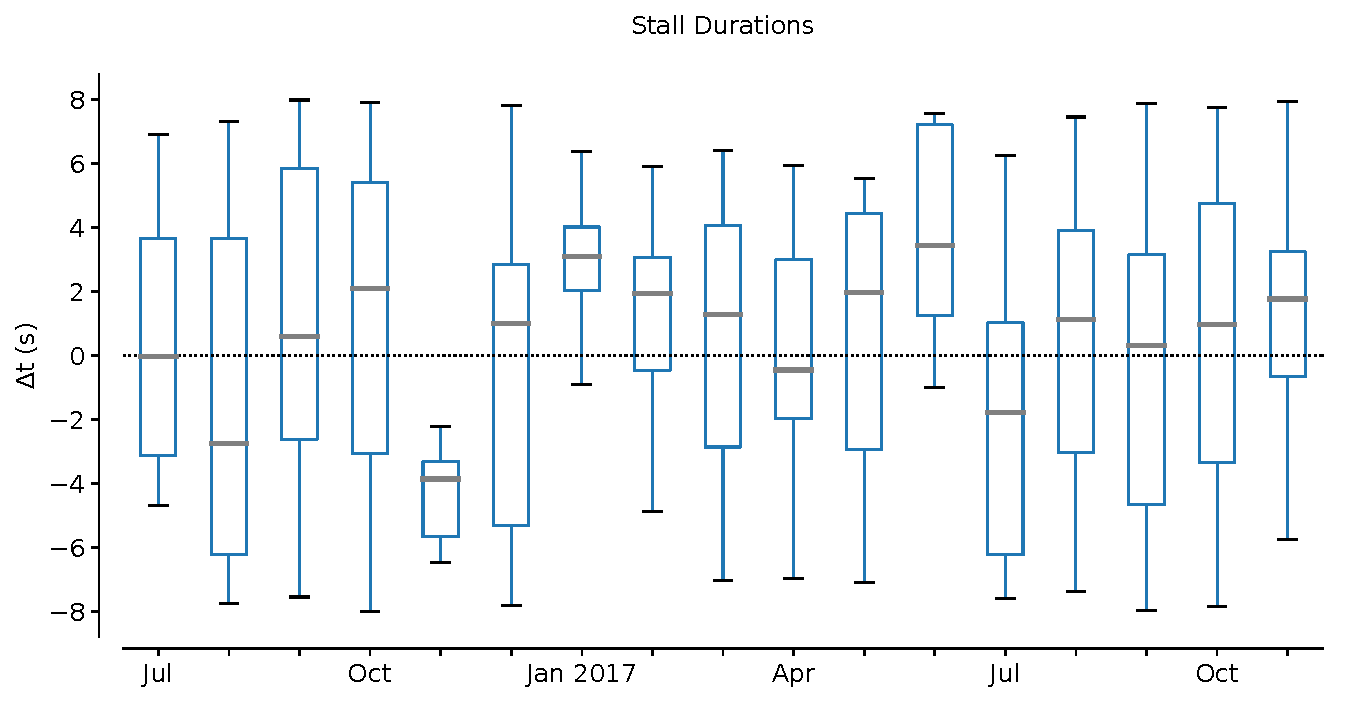
\includegraphics[keepaspectratio, height=5cm, width=15cm]{figures/stall/netflix-stall-durations-diff-box.pdf}
	\caption[Boxplot of difference of stall durations over IPv4 and IPv6]{Boxplot of difference of stall durations over IPv4 and Ipv6. It shows the similar characteristics as in \cref{fig:Stall Duration Boxplot for IPv4 and IPv6} and we can see the variation between different months.}
	\label{fig:Stall Duration Difference Boxplot}
\end{figure}
\begin{figure}[!ht]
	\centering
	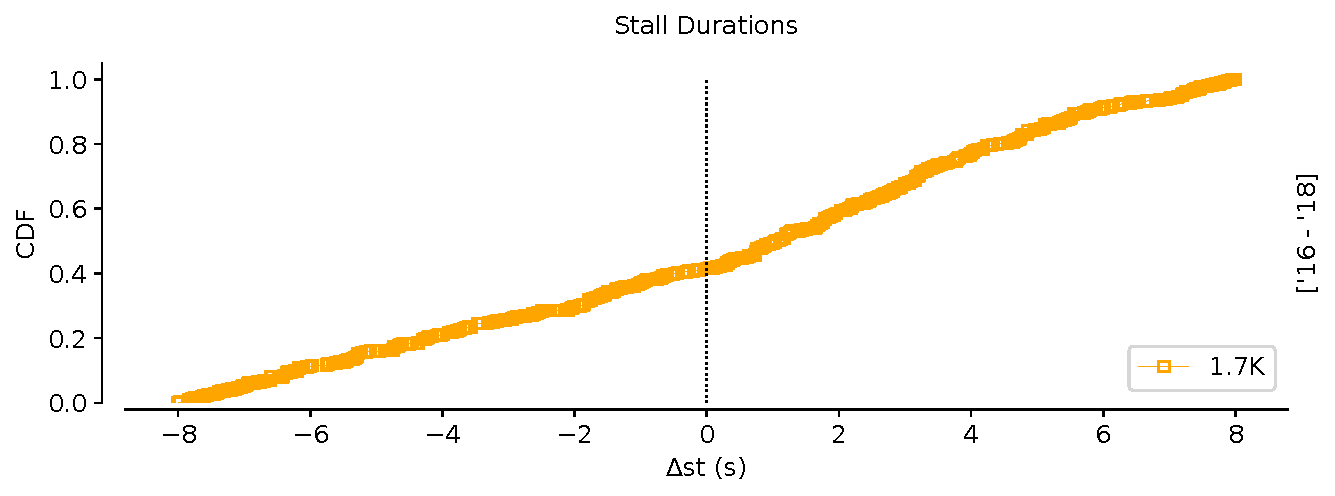
\includegraphics[keepaspectratio, height=4cm, width=15cm]{figures/stall/netflix-stall-durations-absolute-difference.pdf}
	\caption[CDF of difference of stall durations over IPv4 and IPv6]{CDF of distribution of difference in stall durations over IPv4 and IPv6. 
	Positive values indicates that stall durations are lower over IPv6. 41\% of the samples experience lower stall durations over IPv4, whereas, 59\% of the samples experience lower stall durations over IPv6 with around 25\% of them at least 5 seconds shorter.}
	\label{fig:Stall Duration CDF}
\end{figure}

\FloatBarrier